\documentclass{article}


\usepackage[utf8]{inputenc}
\usepackage[left=1in,right=1in,bottom=1in]{geometry}
\setlength\parindent{0pt}
\setlength{\parskip}{1em}
\setcounter{secnumdepth}{0}
\usepackage{outlines}
\usepackage{hyperref}
\usepackage{graphicx}
\graphicspath{ {imgs} }

\title{Urban Social Geography}
\author{Carla Hyenne }

\begin{document}

\maketitle

\tableofcontents

%%%%%%%%%%%%%%%%%%%%%%%%%%%%%%%%%%%%%%%%%%%%%%%%%%%%
%											LECTURE 1
%%%%%%%%%%%%%%%%%%%%%%%%%%%%%%%%%%%%%%%%%%%%%%%%%%%%

\pagebreak\section{Urban Geographical Traditions}
\date{September 27th, 2021}

Draw a general outline of how urban geography has been practiced in the last 50 years, and how it interrogates some of urban geography's main concepts and approaches.

\subsection{What is "the urban"?}

\subsubsection{Urban Age}

We are living in the Urban Age, where the population growth is proportional to urban growth. Since circa 2005, the majority (more than 50\%) lives in urban areas, or cities, as opposed to rural areas.

Urbanization is a \textbf{global phenomenon}. It started with the global North (USA, Western Europe) in the 19th century, spread to South America, USSR, Oceania in the 1950s, and Africa, Asia in the 1990s. Urbanisation intensified in the 1990s, and as of the 2000s, Asia dominates the economic growth and urbanisation.

Urbanization isn't equal throughout the world. For example, in 2018, ~40\% of Africa's population was urban, ~50\% in Asia, ~75\% in Europe, ~80\% in Latin America and North America, and ~70\% in Oceania.

\begin{center}
	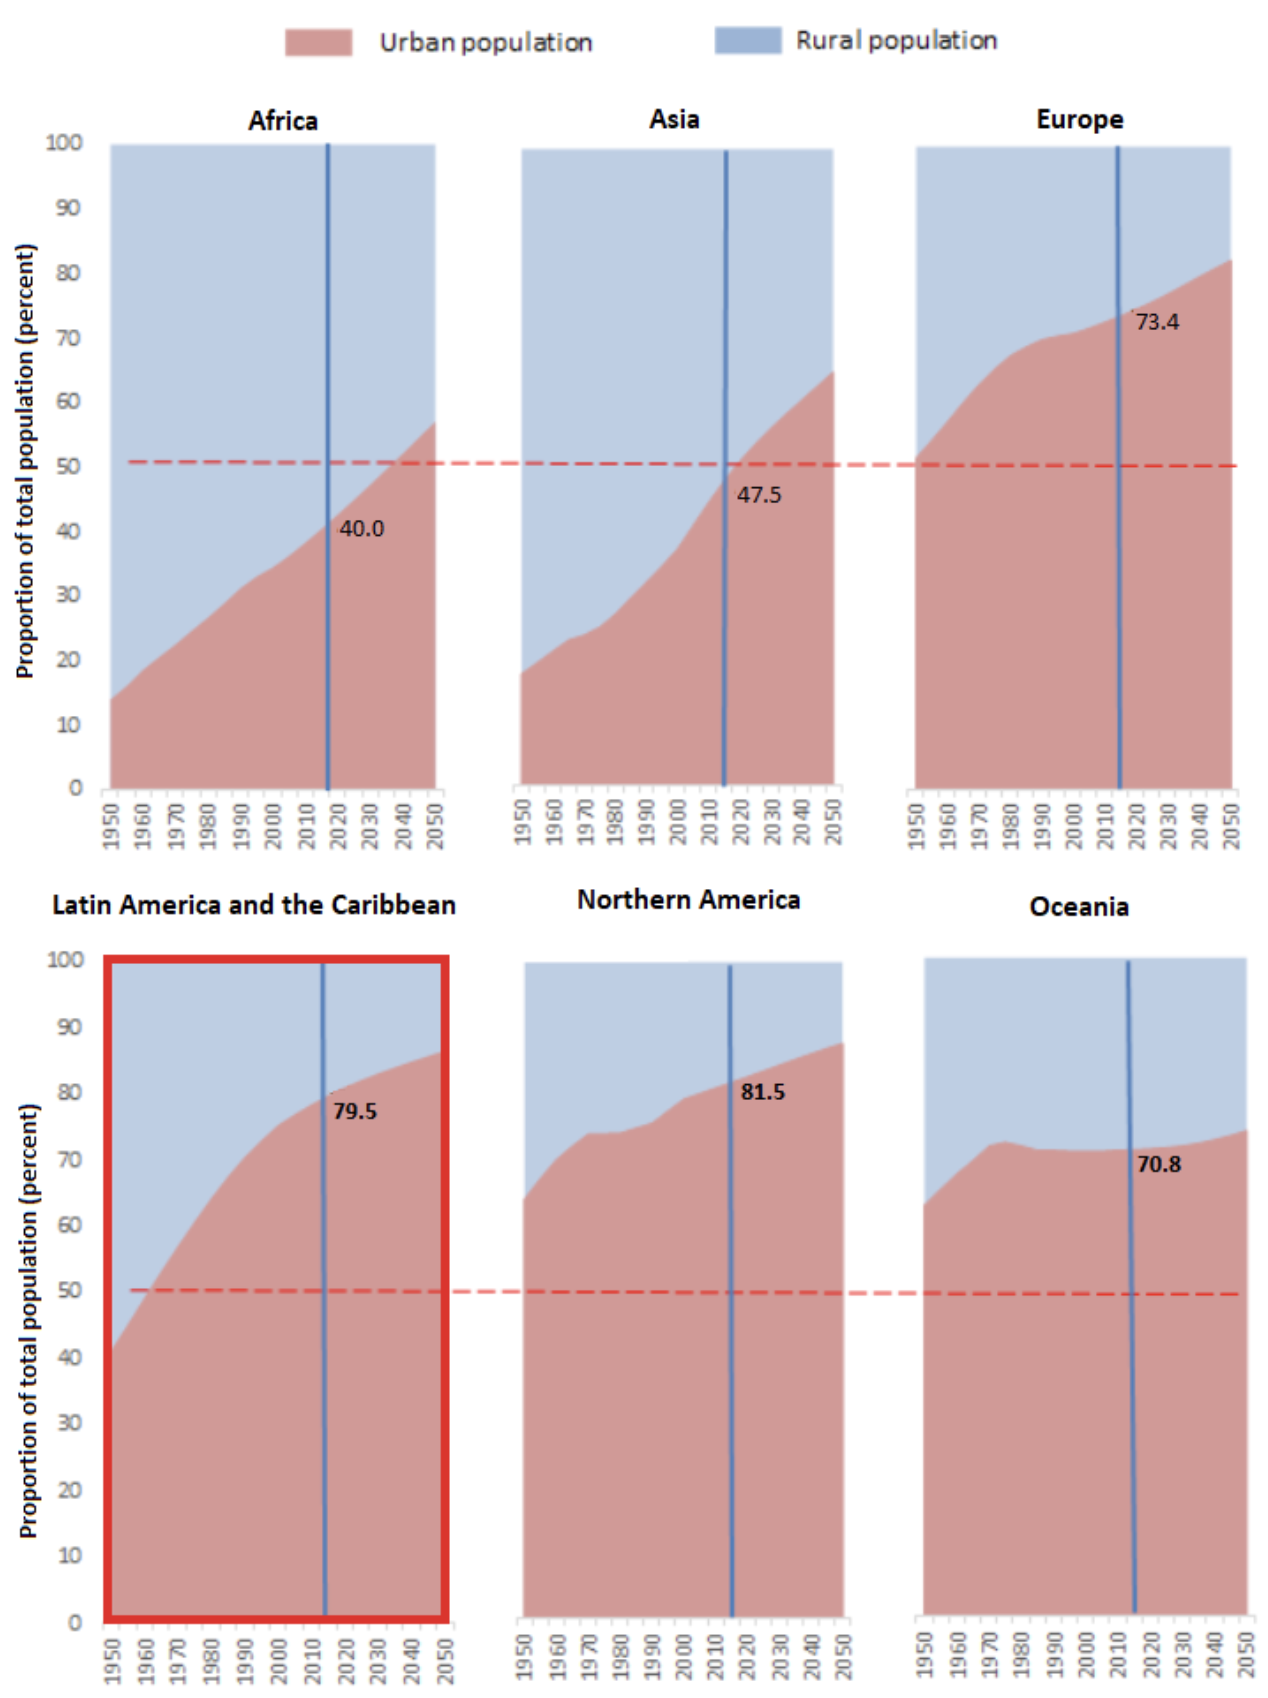
\includegraphics[width=30em]{urban_rural_proportion}
\end{center}

Is urbanization really "global"? Are we really in an "urban age"? How we measure the urban depends on statistics and national definitions and categories that diverge. It is impossible to find one definition of the urban. What is understood as "the urban" is a \textit{chaotic abstraction}, and doesn't neatly overlay cities in the spatial sense (boundaries). 

This makes the distinction of the urban vs. the rural, and the categorisation of space in either or, a black box. Is it important to think about the rural? What is difference between the urban and the city?

\subsubsection{What is the difference between the urban and the city?}

The urban is a phenomenon, a process, and elements of the urban can exist outside of the city. 
It is a set of values which direct how we might organise a city.

The city is a built environment, made of concrete. It is a marker in space, it is a physical manifestation of the urban. 
It has boundaries and is political - cities have mayors and elections, for example.

Thus, the urban is greater, theoretically, than the city.

\subsubsection{Urban Conceptualisations}

\begin{itemize}
  \item A distinctive way of life, which can take place in cities but also outside of the city (suburbs, rural, slums)
  \item It epitomises a particular society (capitalist, industrial, fordist, modern, classist...). The urban can therefore be categorised differently depending on the context and time period. 
  \item Projects symbolic power (see city conceptualisations)
\end{itemize}

\subsection{What is "the city"?}

\subsubsection{City Conceptualisations}

\begin{itemize}
  \item A lump of material, the \textbf{built environment}
  \item The non-city is... what? the rural? It is hard to say where the city ends. For examples, large boulevards connecting the city to "outside" spaces may have shops along them, which could be characteristic of the city. But are they still part of the city?
  \item A complex division of labour, with increasing efficiency and surplus, but also inequality
  \item Projects symbolic power, through skyscrapers and impressive architecture that reminds the world of the city's social/political/economic dominance. Think of the CCTV tower in Beijing, World Trade Center in NYC, Burj Khalifa in Dubai. But what is behind this image of spectacular urbanism? Is it a facade?
  \item Is administrative, with administrative boundaries
\end{itemize}

\subsection{The Urban as a Process: Urbanisation}

Urbanisation is:

\begin{enumerate}
  \item \textbf{Demographic process} in which cities gain more and a wider variety of residents, with an increased density
  \item It speaks to the increasing \textbf{globalisation of urban economic, political and cultural influence}
  \item It helps us consider \textbf{how space is organised} through processes of uneven development
\end{enumerate}

Urbanism is:

\begin{enumerate}
  \item Narrowly defined as \textbf{urban design}
  \item Gaining an \textbf{urban attribute}, a psychological and sociological feeling, giving particular meaning to urban space. \textit{Flaneurs, dandys}
\end{enumerate}

Planning is:

\begin{enumerate}
  \item A future-oriented activity, where actors of various types engage to govern how development will take place
\end{enumerate}

\subsection{What is "geography"?}

Geography is the terrain, the typologies, the interconnectedness of space and 'something' within that space; the \textbf{social and physical processes within the context of space}.

Geography is defined by "how" we study, rather than "what", with an emphasis on space. There are different concepts of space: territory, scale, place, and networks.

The \textbf{territory} defines boundaries, and sovereignty of a space (the Brussels capital has sovereignty within Belgium). 

The \textbf{scale} defines the sensitivity of processes (teaching is a small scale, commuting is a large scale, the Brussels capital scale is greater than its territory). 

The \textbf{network} defines hubs and leaks beyond the territory, towards micro-networks (Brussels connected to other cities via a transport network, but also by people living in eg. Ghent and commuting to Brussels to work. This is a leak of taxes and money from the capital to Flanders/Wallonia)

The \textbf{place} is the attachement of meaning, sentiment, to a place (how Brussels is represented in Flemish vs. Wallonia media)

\subsection{What is being "critical"?}

To be critical is to be aware of your own biases, and not cherry-picking your information. To be critical is to fact-check and question, to be reflexive about your own positionality. You should bring up new concepts, and take seriously the experience and position of others. Critical research should be socially relevant and politically engaged. The Chicago School would define it as \textit{"reducing the illusions in society itself"}.

Brenner and Schmidt are critical authors of the Urban Age.

\subsubsection{Epistemological Rules of Thumb}

\begin{enumerate}
  \item There is no universal theory of anything
  \item Every theory has birthmarks: what were the questions, situated in time and space, that gave rise to formulating a search question/theory in a particular way?
  \item Reflexivity on birthmarks is required if you want to be critical, therefore all theories need to be provincialised
  \item Can theories "speak" across contexts?
  \item Engaged pluralism might allow for inter=theoretical conversation and comparison
\end{enumerate}

\subsection{Foundational Approaches}

After WWII, geography moved from purely territorial to plural definitions, from regional (urban) geography (descriptive, map-oriented, idiographic) to a spacial science (nomothetic, method-driven, applied orientation).

The \textbf{materialist approach} has materialist frameworks, is concerned with distribution and social-justice, and agenda-setting: Marxist geography, Structuralist geography, Critical geography, Radical geography, Feminist geography, Critical realist geography

The \textbf{humanistic approach} is about the experienced city, issues of representation and discourse, uses qualitative methods, and is about giving voice: Humanist geography, Cultural urban geography, Post-structuralist geography, Post-colonial geography, Queer geography

%%%%%%%%%%%%%%%%%%%%%%%%%%%%%%%%%%%%%%%%%%%%%%%%%%%%
%											LECTURE 2
%%%%%%%%%%%%%%%%%%%%%%%%%%%%%%%%%%%%%%%%%%%%%%%%%%%%

\pagebreak\section{Theories of world-city formation}
\date{Octobre 4th, 2021}

The first session on world and global cities aims to:
\begin{itemize}
  \item Provide a framework to conceptualise and analyse cities under (economic) globalisation
  \item Give an overview of key theories of world-city formation dating back to the 1970s-1980s and onwards
  \item Introduce model-based approaches to the world-city network as a heuristic to map out how cities are positioned on global flows of capital, knowledge, and people
  \item Discuss a number of key critiques of the alleged "world/global cities paradigm", voiced from social constructivist and post-colonial positions
\end{itemize}

\subsection{Centrality of cities/city-regions in the global economy: Friedmann, Sassen, Scott}

How are cities central in the global economy? What does it mean to say that cities are powerful? 

\begin{outline}
	\1 Concentration of businesses, seats of corporate power, migration of elites to the city
	\1 Cities are administrative and political authorities
	\1 The city is a hub of ideas, culture, social influence, and knowledge transfer
	\1 Flows converge in cities, and flow between big cities: it's easier and faster to travel between cities than from a city to its periphery or towns. The substance of the flows can be knowledge, people, capital, commodities
\end{outline}

The five most powerful regions of Europe are Deltametropolis, Flemish Diamond, RheinRuhr Area, Ile-de-France, and Greater London.
There are multiple ways that we can measure the power, or influence, of such world-cities:

\begin{outline}
	\1 \textbf{Weight of area in national context}: the \textbf{GDP} is higher, and the density of population is higher\footnote{Higher than the European and national averages. This applies to the rest of the indicators.}
	\1 \textbf{Patents}: number of patents is higher. This indicates the level of social and technological innovations of a city
	\1 \textbf{Education}: the proportion of people educated at a high level is higher. This indicates a different labour market structure
	\1 \textbf{Employment by sector}: proportion of employment in services is higher, and proportion of employment in industry or agriculture is lower
\end{outline}

\subsubsection{John Friedmann, \textit{World City Hypothesis}}

\textit{tldr; global cities are basing points in a global (economic) urban system, organising and articulating production and markets}

\textbf{Why are cities economically central and powerful?}

There were predictions in the 1980s that ``the end of the city" was coming, due to ICT and cheap mass transportation. Instead, these gave rise to new forms of uneven development related to \textbf{functional centrality} on a more global scale. People could travel from further distances and still work in the functional (city) centre, and have relationships with people from a longer distance.

World cities were inserted in a \textbf{global urban system}, in which urban processes that cross-cut national and regional borders are conceptualised: this insertion drives structural change in cities and renders some places powerful. We have to look beyond national urban systems, and start thinking about processes of \textbf{globalisation}, ie. on a global scale. A great part of economics became international, and only the global urban system can explain what is happening internationally. 

In this sense, world-cities are the base points to explain ``spatial organisation and articulation of production and markets'' (\textit{The World City Hypothesis}, Friedmann, 1986), ie. the geo-economic restructuring of the world.

There is a new \textbf{international division of labour} in the world. Companies offshore their production activities or relocate to (semi) peripheries to drive prices down because of cheaper labour markets, in order to stay competitive. There are new actors, TNCs and MNCs (trans- and multi- national corporations) that dominate and organise a global supply chain that is highly integrated\footnote{This complex, interconnected division of labour is illustrated by 1) the Evergreen container ship that blocked the Suez canal and blocked distribution of goods for a week, or 2) the lack of bicycles during the covid pandemic, when manufacturing plants had to close due to regional or national safety measures.} Given the importance of TNC/MNCs, mapping their headquarters can be used to locate world-cities. 

This illustrates that world-cities are sites for centralised \textbf{command and control} functions in a complex global economy. It implies a hierarchy connecting the core and the periphery, with core cities absorbing the surplus (and thus getting richer and growing in all dimensions)\footnote{This means that locations and cities will benefit unequally from this geography: the US (Global  North) producing in Argentina (Global South) will benefit the US, who extracts the profit, and disadvantage Argentina, who has a cheaper labour market}. But, (semi) peripheries can still hold local command and control functions.

\subsubsection{Sassen, \textit{The Global City}}

\textit{tldr; global cities are cities where APS (Advanced Producer Services) are produced for the international market; APS have control capabilities over global production, and they produce global financial markets}

Sassen writes at the same time as Friedmann, in a context of de-industrialisaiton (specially in NY, London, Tokyo) and fiscal crisis of the local state, and cities are trying to figure out what they might become.
Sassen focuses on the \textbf{shift to service economies}, especially finance services and auxiliary services in law, management consultancy, accounting, auditing, advertising, etc. These auxiliary services are called \textbf{advanced producer services (APS)}, they are not producing consumable goods, but rather goods that are consumed as they are produces (eg. legal advice).

Advanced producer services are embedded in global cities, and they have \textbf{control capabilities} to manage global production and produce global financial markets. There is a \textbf{labour market polarisation}, with high and low skilled labour forces surround APS, which results in the ``peripheralisation'' of the core (eg. sweatshops).

Sassen says that \textit{``global cities are sites for the production of specialised services needed by complex organisations for running a spatially dispersed network of factories, offices, and service outlets; and the production of financial innovations and the making of markets, both central to the internationalisation and expansion of the financial industry''}.

Global cities are connecting to the world of finance for investments, and growing the need for concentration and control. This geography is self reinforcing.

Why are APS concentrating in a limited number of cities? There are several interlocking \textbf{path dependencies}:
\begin{outline}
	\1 \textbf{Large services market}: there is access to firm/client relations, for out-sourced APS
	\1 \textbf{Labour market and associated culture}: a cosmopolitan elite and `yuppie' (young urban professional) culture is formed, since the 1980s
	\1 The most specialised and globalised APS firms need \textbf{synergies} with similar firms in the city, which creates an \textbf{APS complex}. For example, financial firms, ICT firms, advertising, management consultancy, accountancy, and legal services all need each other to some extent
	\1 The APS complex produces \textbf{cross-border connections} through a network of affiliates and other partnerships
\end{outline}

Even within the city, there are APS clusters. For example, the concentration of law firms in Avenue Louise and in the EU quarters of Brussels.

\subsection{Scott, \textit{Global City Regions}}

\textit{tldr; global city-regions are a complex assemble of cities/settlements/hinterlands that are interconnected via production networks, themselves oriented towards global economy}

Sassen's views of global cities as APS centres fits London, Hong Kong, Brussels, etc., but there are large-scale territorial entities like the Pearl River Delta\footnote{One of the most densely populated urban regions of the world, considered a megacity, and one of the wealthiest regions in China.} and the Bay Area, which have global power but are not cities. Many production processes don't need an `urban core'.

The need for centrality is applicable to \textbf{post-Fordist modes of production\footnote{Post-fordism is the idea that modern industrial production has moved away from mass production in huge factories, towards specialised markets based on small flexible manufacturing units}, where knowledge is central}. The concentration is a by-product of globalisation and technological innovations (cf. cognitive-cultural capitalism). 

So, not only APS need to be centralised. For knowledges that are not easy to de-centralise, proximity matters. For example 1) industries in which it is important to communicate with clients face-to-face, or 2) tailored, just-in-time delivery. Concentrating an activity in one area also makes it easier to receive federal/public investments (ie. investments drive centralisation).

\textbf{Global city-regions} are a complex ensemble of cities/settlements/hinterlands, that are interconnected via multiple production networks, which in themselves are oriented towards the global economy. APS firms can still be used as a general indicator of the globalisation of Global City-Regions, as they produce the tools to enable proper functioning in a global economy.

\subsection{Mapping world city networks}

Comparing the importance of urban connections (eg. London/Hong Kong vs Paris/Tokyo) is difficult when using available data sources, and without using a secondary data source or creating new data.
This is because there is a research gap regarding world-city networks.
Secondary data could be information on inter-city transportation or information flows (eg. flows of airline passengers). New data collections could be developing a methodology to use specific attribute data to assess inter-city relations (eg, the GaWC-heuristic).

Are airline flows a good way to measure global economic influence, and thus helpful to map the world-city network?
\begin{outline}
	\1 Some cities which are not global-cities have airports, and maybe vice versa
	\1 People travel for leisure, which may tell us something about the local economy but not about the influence of the city's economy on a global scale
	\1 A lot of goods are moved by other means than air, eg. water or land
\end{outline}

Therefore, we need a \textbf{new metageography} of spaces of flows. This would be a new socio-spatial structure.

The GaWC (Globalisation and World Cities) heuristic is an example of a new way to gather data\footnote{See \url{https://www.lboro.ac.uk/gawc}}. The starting point is the presence of international APS firms, that is used as a general indicator for command and control functions of cities. Since APS firms have office networks that comprise of the most important cities in the global economy, we make the core assumption that inter-city relations can be assessed based on the APS firms being present in multiple cities. $\rightarrow$ we measure the connectivity of cities.

APS don't represent all of the global economics, but they represent strategies of the command-and-control of APS firms. 

\subsection{Critiques and complementary views}

The GaWC heuristic is a powerful tool to map and spatially analyse the global connections of world/global cities, but has been criticised from various angles: post-colonial, social-constructivist, political-economy, and financialisation perspectives.


\begin{outline}
	\1 \textbf{Post-colonial critique}: there is a western bias in the knowledge production of urbanisation, people are dropped off the map of urban studies research. 
		\2 Off the geographical map refers to (world) cities in the Global South
		\2 Off the conceptual map refers to the focus on a limited number of economic processes, and ignoring equally important inter-urban connections
		\2 World cities research ignored the role and position of `ordinary' cities in the global economy,  or reads them in light of Eurocentric global city theories 
		\2 Tendency in urban studies to reject world/global city theory as only befitting the Global North, but not on the basis of a sound argumentation: non-representation as a `result', not a `neglect'
	\1 \textbf{Social-constructivist critique}: stresses the political natural of world-city formation and its often un-debated consequences
		\2 Post-modern knowledge theory: world cities are not a `given' but a product of global and local forces, and crucially mediated by acts of representation
	\1 \textbf{Financialisation}: GaWC heuristic is a powerful shorthand for the geographies of world/global cities, but world-city functions are often assumed instead of researched 
		\2 etc...		
\end{outline}

\subsection{Key words}

World cities
World city-regions
Global urban system, global economic system
GaWC
Command-and-control function of cities

%%%%%%%%%%%%%%%%%%%%%%%%%%%%%%%%%%%%%%%%%%%%%%%%%%%%
%											LECTURE 3
%%%%%%%%%%%%%%%%%%%%%%%%%%%%%%%%%%%%%%%%%%%%%%%%%%%%

\pagebreak\section{Polarisation in World/Global Cities}

This second session on world and global cities discussions the connections between the positionality of cities on global circuits of value and their internal social and economic structure:
\begin{itemize}
  \item Applies Harvey's framework to analyse urban  entrepreneurial export-base enhancing strategies
  \item Focuses on the polarisation debate, which has centred on the mechanisms that produce income \& professional divides, the contextual factors that mediate such polarisation processes, the role of high/low-skilled migration, gentrification, etc.
\end{itemize}

\url{https://www.youtube.com/watch?v=qOP2V_np2c0&ab_channel=RSA}

\subsection{Polarisation}

\textit{tldr; polarisation is a class division that is reproduced through space, and is stronger in global cities}

Income disparity looks different in different cities. Chicago, Detroit, LA, Miami, New Orleans, SF, NYC, all have different, contextual landscapes of polarisation.

Polarisation is the reality of \textbf{class division}. \url{https://www.opportunityatlas.org} is an income map that traces neighbourhood effects, based on census data. The \textbf{neighbourhood effect} is the idea that where you are born, predetermines your life. This is due to the amenities, infrastructure, opportunities associated to the geographical location.

Polarisation is one of the starting point of debates in global cities: it raises the questions about \textbf{how class divisions in cities are reproduced in/through space, but also why there is a deep polarisation in key nodes in the global economy}, ie. in world/global cities.

Picture LA, a `citadel' city where polarisation/segregation are both horizontal and vertical (there are no wealthy people residing on the ground floor). Wall Street in LA is a poor neighbourhood in decline, or a `zone in transition', yet it is contrasted with nice hotels. This says to people that `those who have nothing to do here, should not be here'.

\subsubsection{New York City}

We can see how NYC's polarisation patterns have evolved in the last decade, since the 2008 recession: \textbf{polarisation and income distribution gaps have increased}. 

The median family income has fallen\footnote{Income can be equated to labour}, and the decline in income is steeper in NYC than in the state of NY. The share of total income going to the top 1\% continues to increase (it only declines during a financial crisis but quickly rebounds), such that the top 1\% own over 40\% of the total income and the income of the lowest household is \texttildelow17.5\% of the top earners' income. And the gap in increasing.

\textbf{Productivity has increased but wages have not}: for 1 hour of work, an extra 14\% is produced, but the wages have not proportionally increased. The profit is not going to the workers, and a full-time worker at a minimum wage now lives under the \textbf{poverty line}.

\begin{center}
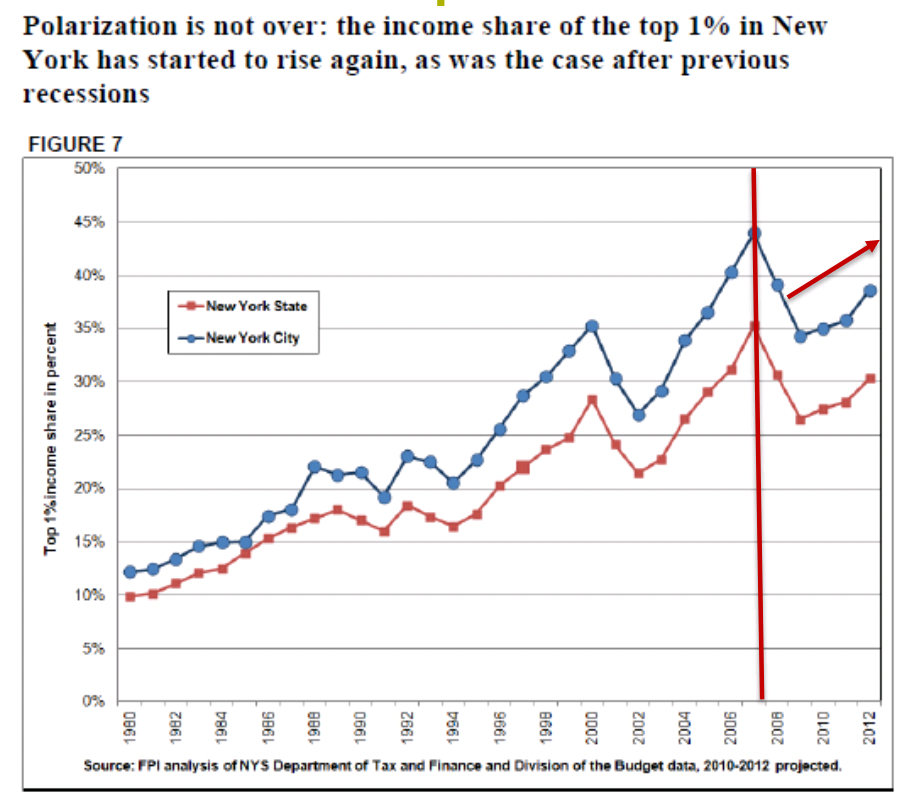
\includegraphics[width=23em]{nyc_income_gap}
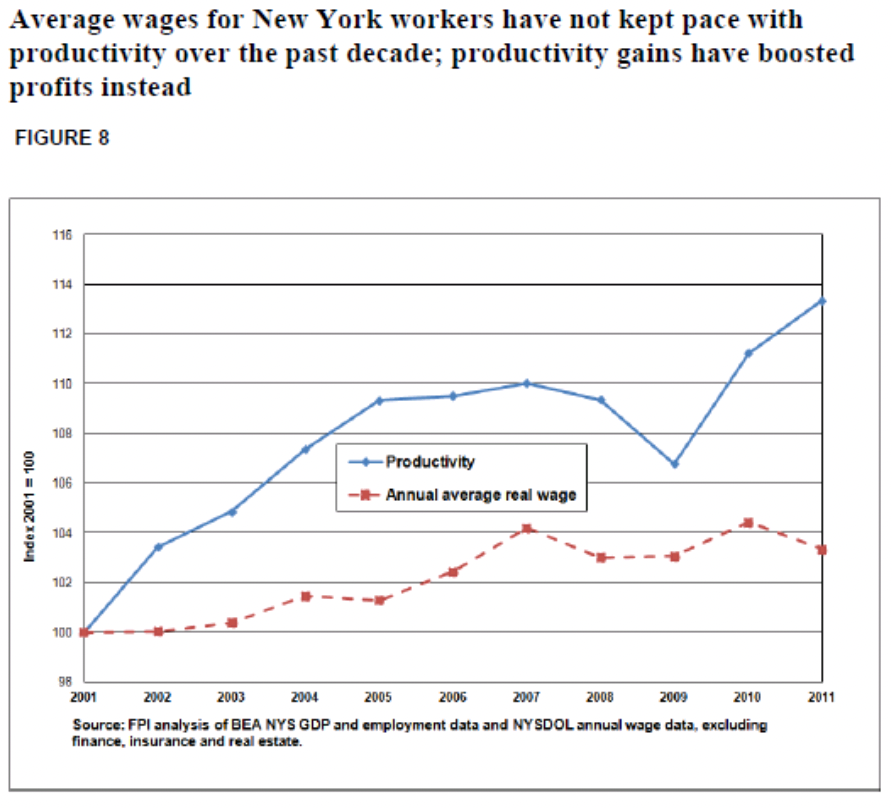
\includegraphics[width=23em]{nyc_productivity_gap}\footnote{Fiscal Policy Institute report, \textit{Pulling Apart: The Continuing Impact of Income Polarisation in New York State}}
\end{center}

\subsubsection{Why is it that world/global cities have become so polarised?}

\begin{outline}
	\1 Large companies with a lot of capital are subsidised
	\1 Unequal income distributions, where rich companies are getting richer
	\1 Companies are looking for the fastest way to make money, ie. they employ at the lowest wage possible. It's a corporate strategy to not care about the general welfare of the workforce
	\1 The state is not taking the role of creating regulation and (welfare) policies
	\1 Extra money ``floating around'' goes into financialisation, as can be seen with the gap in productivity (profit) and wages 
	\1 Companies can remove workers who want higher wages, because there is enough demand for such low-wage jobs
	\1 A worker needs to be produced in a ``social way'', including education, health,... (social reproduction) which happens in cities
	\1 Poverty blaming does not help with polarisation, eg. Benefit Street
\end{outline}

\subsection{Conceptualisation}

The main explanation for why polarisation exists, is because of economic restructuring (this is mostly about North-Atlantic cities).

Some conceptualisations:
\begin{outline}
	\1 ``Dual cities'', Mollenkopf and Castells, 1991
	\1 ``Divided cities'', Fainstein et al., 1992
	\1 ``Quartered cities'', Burgers, 2002
	\1 ``Polarized cities'', Sassen, 1991; Friedmann 1986
\end{outline}

\subsubsection{Economic restructuring}

The crisis of North-Atlantic Fordism in the 1970s led to an economic restructuring. With Fordism, there was a deal between the companies and workers, that they would get a wage allowing them to purchase the items they were manufacturing. However, productivity couldn't keep up with wages\marginpar{i don't understand}. This entailed:

\begin{outline}
	\1 \textbf{A relocation of production}, ie. offshoring and decentralisation made possible by \textbf{globalisation and the new international division of labour} (NIDL)
	\1 \textbf{The deindustrialisation of the core}: production activities in cities declined
	\1 \textbf{Structural unemployment}: as cities lost their functions, poverty rose and became characteristic of cities
	\1 \textbf{Shift towards fiscal austerity}: the tax base declined
	\1 \textbf{Market rationality and privatisation}: the state interfered less and encouraged privatisation (market deregulation which enriched companies), and shifted towards neoliberalism (Thatcher, Reagan)
	\1 \textbf{Declining power of the state to control multinational capital}: this power shifts to multinational companies
	\1 \textbf{Self fulfilling prophecy of interurban competition}: policy makers are trying to become entrepreneurial, and instead of being fair, start to be competitive
\end{outline}

Harvey (1989) proposes four ``entrepreneurial'' strategies to navigate this crisis: production, consumption, redistribution, command and control

\subsubsection{Production}

Policy makers create or exploit particular advantages for the production of goods and services:

\begin{outline}
	\1 Attracting public and private investments into physical and social infrastructure, to strengthen the economic base 
	\1 Stimulating new technologies, venture capital...
	\1 Reducing local costs with tax breaks, cheap credit...
	\1 Reducing ``excessive'' labour costs or investing in highly educated labour force
	\1 Stimulating a mix of related activities and creating agglomeration economies, eg. Silicon Valley
	\1 \textbf{Form}: clusters and edge cities
\end{outline}

\subsubsection{Consumption}

The city's position in the spatial division of consumption should be improved:

\begin{outline}
	\1 Make people want to spend money in your city: through tourism, retirees, local consumers
	\1 Residents rarely see an increase in their wages, despite the attraction of money in their city
	\1 There's an increased credit, and a dependence on banks to finance consumption
	\1 Attract high income jobs (managerial, CEO...) and their conspicuous consumptions
	\1 \textbf{Form}: the socio-spatial structure is affected by consumerism, visible by gentrification, cultural innovation, upgrading of urban environment (starchitecture), consumer attractions, spectacle, heritage, city branding/marketing
\end{outline}

\subsubsection{Redistribution}

There is a competition for the (supra)nationally distributed surplus. Cities and regions compete with each other to attract investments. The surplus comes from the economy, and not the government budget. Especially under austerity, which cuts government budget and makes the surplus allocation problem greater.

Who competes for surplus?

\begin{outline}
	\1 Military/defense investments in the US
	\1 EU countries for EU money
	\1 Urban renewal projects in Flanders
\end{outline}

\subsubsection{Command and Control}

A specific kind of investment in connectivity, to assume control in high finance, government, and information gathering/processing:

\begin{outline}
	\1 Investment in connectivity infrastructure, both physical and digital
	\1 CBD-development and office space strategies
	\1 Investment in high-skilled labour markets and education (universities, business schools,...); companies sponsor finance programs for employees
	\1 \textbf{Form}: a dynamic in world/global cities and their monopoly spaces (eg. Wall Street, the City of London)
\end{outline}

\subsection{Polarisation thesis}

Main authors are Friedmann \& Wolff (1982), Friedmann (1986), Sassen (1991)

The key trend is the change in economic base, leading to a decline in well-paid manufacturing jobs (exodus) and a growth in service jobs (formal/informal).

This entails an influx of high salaried people, with high spending power (the highly-skilled, highly-paid, upper circuit, upper social strata). This in turn generates a demand of low paid jobs to cater to them  and their conspicuous consumerism (low skilled, low paid, underclass, the remaining social stratum).
This transforms the labour market, such that there is a growth of \textbf{jobs at the top and bottom} of the job ladder, but a decrease in demand for jobs in the middle. The informal economy and informal workers also grow.

\begin{center}
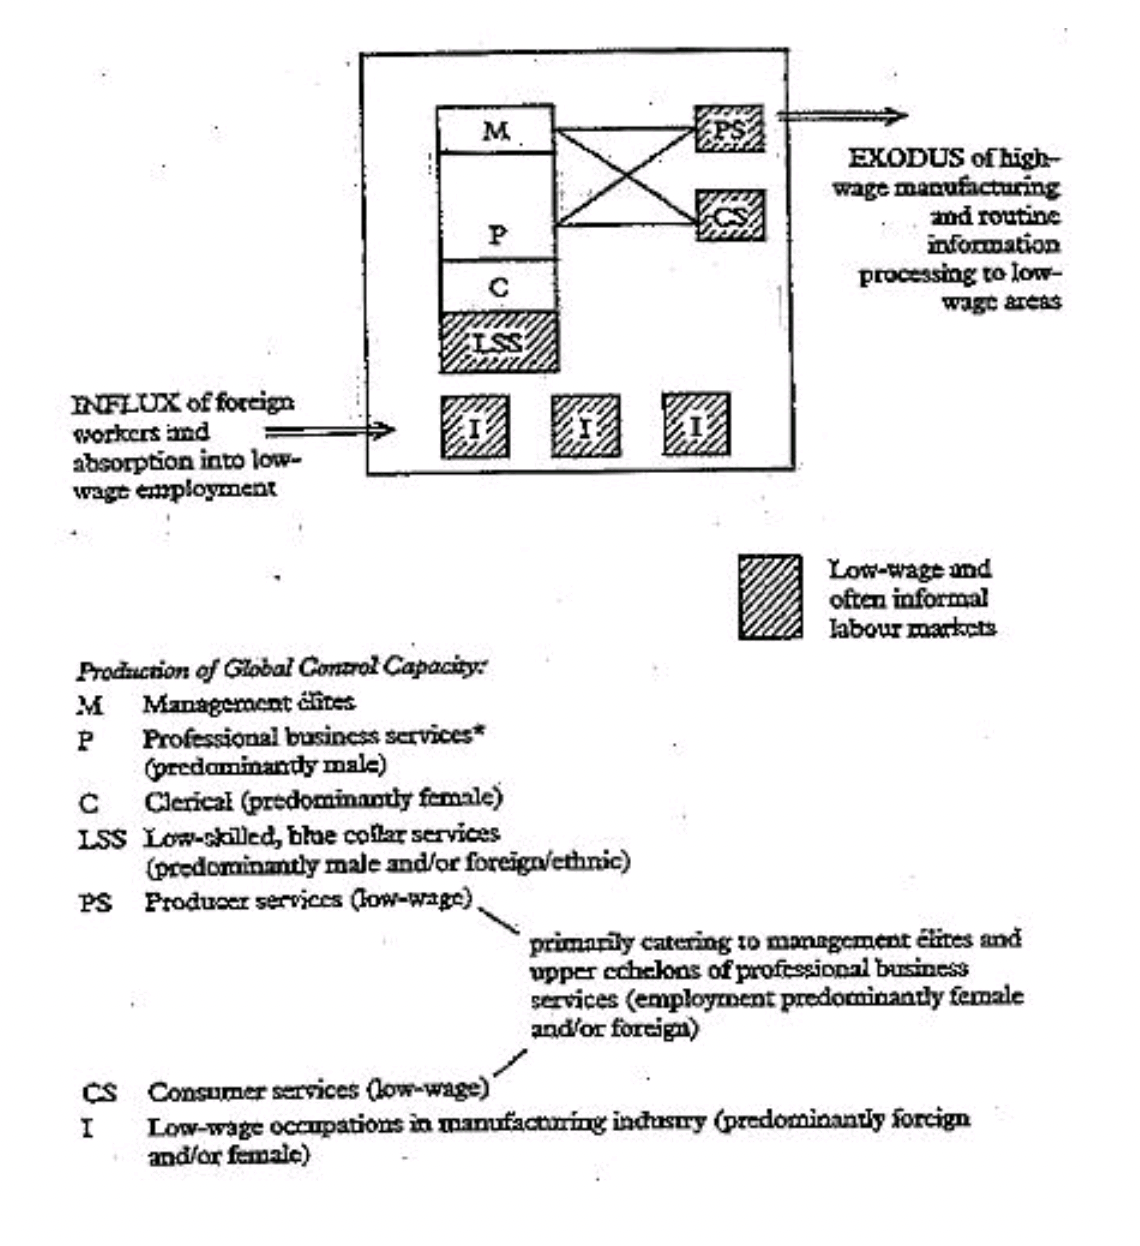
\includegraphics[width=40em]{polarisation_thesis}
\end{center}

\subsection{Labour Market Globalisation}

What sets global cities apart is their \textbf{globalised labour market}. There is a growing role of high-paid and low-paid migrants in the urban economy, this divide is often articulated along ethnic lines (``expats''\footnote{Debate in Belgium about how to tax expats, who currently enjoy a low tax rate} vs. ``immigrants'').

The growth of the supply of low-skilled/deskilled workers causes a downward pressure on wages. These are people who did not have, or no longer have (ie. having lost, or not recognised) qualification from their country of origin.

This creates a large pool of people who do not have power to make demands on their wages, and the pool is large enough that workers can be replaced by others who are willing to work for these low wages.

An example of low-skilled jobs are \textbf{3D jobs} (dirty, demanding, dangerous/difficult) originally were paid higher wages in order to attract workers. Now, low-wage jobs are for those otherwise excluded from the labour market.

There is growing \textbf{informality and ``peripheralisation at the core''} (Sassen-Koob, 1982). Exploitation does not only take place in the Global South: it also takes place in the Global North (ie. the global cities, the core) where people from the Global South (the peripheralised) live.

Immigration lead to the expansion of `informal', `floating', or `street' economic activities, such as sweatshop manufacturing, off-the-book childcare, and other unregistered, non-taxpaying activities. You need some knowledge to be able to access the market place, or you are excluded and must find informal work.

\subsubsection{Urban Elite Networks}

A way of measuring the connection between cities, by looking at the membership overlaps across the board of directors (one member sitting in multiple boards).
 
 \subsubsection{New forms of industrial exploitation}
 
Sweatshops are reminiscent of old-forms exploitation. They are small units in secluded spaces, they function with subcontracted deals which makes it hard to know who is actually contracting, and workers are paid by the pieces or by weekly contracts. This is highly precarious work and hard to regulate.

Sweatshops have re-emerged in the new industrialisation age (20-21st century), which is made possible by the absence of labour rights protection. They are always located in the global peripheries.
 
\textbf{Thus, global city formation is made possible by the absence of regulation in the periphery.}
 
\subsection{Criticism}

The two main criticisms are:

\begin{outline}
	\1 \textbf{Universalising and generalising tendencies}: started in London, NY, Tokyo, and is considered universal, but is it the case? 
		\2 The thesis projects this logic: economic restructuring + globalisation $\rightarrow$ HQ + APS functions $\rightarrow$ income + professional polarisation $\rightarrow$ socio-spatial polarisation
	\1 \textbf{Simplistic theory}: polarisation theory is elegant but reduces the complexity of what is going on. Occupational and spatial structures need to be studied in detail. Professionalisation and mobility could also help explain socio-spatial inequalities
\end{outline}

\subsection{Occupational Structure}

\textbf{Polarisation vs. professionalisation}: London's high-income jobs are growing, but this is not necessarily combined with a growth of low-paid jobs. The reason is that the labour market is ``upgrading'', such that people with the required qualifications for highly skilled jobs are moving up the social ladder, which expands, not declines, the middle class.

Plus, a more generous welfare state curbs extreme polarisation (eg. no sweatshops, presence of minimum wage).

The main source of inequality emerges from labour market \textbf{exclusion} and how labour markets intersect with \textbf{gender and ethnicity}. For example (in NY and London), the upper stratum of the executive and professional is dominated by white males; racial and gender discrimination is restricting access of certain groups to highly paid jobs even if they possess required skills; ethnic groups are concentrated in specific parts of the economy, third of London's Filipino population is in health/social care, and Brazilians in cleaning services.

\subsection{Spatial Structure}

\begin{outline}
	\1 To what extent is polarisation a statistical artefact?
The middle class is \textbf{suburbanising}, so maybe the middle income job disappearance is an of artefact as suburbanisation, and thus the entire metropolitan area needs to be taken into the analytical scale, not just the city centre $\rightarrow$ scale matters
	\1 Higher incomes drive demand for high-end housing. This ignites a process of a return to the city and ultimately, (super) gentrification pushing out middle classes
		\2 Brooklyn
		\2 Brussels' evolution of migrant populations: the Moroccan population has grown in the north-west ``poor crescent'', but Europeans and expat populations have grown in the south-east part of city. This is caused by Belgian policies, which promoted Brussels to North Africans as a prosperous city; when industry declined in Brussels, the immigrant families concentrated in the north-east.
	\1 Occupational and income restructuring can take many spatial forms. Need to look at pre-existing structures of the city and its path-dependencies
\end{outline}

\subsection{Three-layer model}

A three-layer explanatory model is required for analysing inequality in cities (Burgers and Musterd, 2000)

\begin{outline}
	\1 Macro-level: a level of global change, referring to economic restructuring, and the increasing mobility of capital, people, commodities and information
	\1 Micro-level: an individual level, referring to the change in labour market opportunities of individuals in a specific local context
	\1 Medium-level connecting the macro and micro-levels, the global and the local
		\2 Subcultural differences among ethnic groups in labour market access
		\2 National institution differences, eg. corporatist social democratic welfare states in Europe provided strong employment protection and benefit systems, which had a moderating impact on the outcomes of economic structuring in the 1980-90s; vs. the liberal welfare state of the USA showed more pronounced levels of inequality due to the loss of jobs and income
		\2 Different urban trajectories, related to urban functions and positionality; industrial towns (eg. Charleroi, Detroit) vs. administrative centres or command-and-control centres
\end{outline}

\subsection{Conclusion}

The gap between the rich and poor is expected to expand. 

\begin{outline}
	\1 \textbf{Austerity}: the permanent state of austerity means stagnating income and declining subsidies, which generates very unstable conditions for lower incomes
	\1 \textbf{Flexibilisation of the labour market}: increased levels of long-term unemployment, and flexible low-wage jobs put a large portion of the population close to the edge of financial insolvency
	\1 \textbf{Migration}: renewal of reserve army of labour through migration, if social policies are not put in place the environment for exploitation will not disappear
	\1 \textbf{Political wealth}: return of patrimonial capitalism, a rentier class banking on wealth and not labour. It matters more who your parents are, your return on investments, than the choice of your profession and your amount of labour
\end{outline}

The function of cities is transforming, and they are becoming `safety deposit boxes' for the people who rely on wealth. For example, in London entire neighbourhoods like Knightsbridge and Chelsea are owned by people who live in the Middle East; Shell companies owning 30 million \$ apartments in Manhattan, to maintain their wealth in a given place, but these buildings are empty.

Thus, de-urbanisation is taking place in global cities, where there are growing numbers of empty shells, and neighbourhoods

%%%%%%%%%%%%%%%%%%%%%%%%%%%%%%%%%%%%%%%%%%%%%%%%%%%%
%											LECTURE 4
%%%%%%%%%%%%%%%%%%%%%%%%%%%%%%%%%%%%%%%%%%%%%%%%%%%%

\section{Urban segregation: patterns and causes}

\textit{October 25th, 2021 - Nick Schuermans}

\subsection{Classical land-use models}

Land use models, or models of urban form. Elements of all these classic models can be identified in many large Western cities.

\subsubsection{Burgess' land use model, 1925}

Burgess was trying to understand what cities looked like, and what kind of groups can be found where.
He found 5 concentric rings: the loop (CBD), zone of transition, zone of working class, suburban zone, commuter zone.

\begin{outline}
	\1 \textbf{Loop, or CBD}: Chicago had an elevated metro track that ran in a loop; place with shopping, offices, HQs, theatres... ie. the functions that are able to pay the highest price for this central location. They need to draw workers/consumers from all corners of the city, thus need to be in the loop
	\1 \textbf{Zone in transition}: factories that rely on labour coming from different parts of city, but who are not able to pay as much rent as the businesses in the loop; also residential, for first generation immigrants who cannot yet afford to live further out (eg. Little Sicily)
	\1 \textbf{Working class zone}: `respectable' working class neighbourhoods (eg. Belgians, Russians, who had been able to climb social ladder and move away from factories)
	\1 \textbf{Suburban zone and Commuter zone}: better, middle-class residences and commuter belt
\end{outline}

The reason there are five rings, is because of the \textbf{bid rent theory}. It explains that different groups of people are able to pay (afford) different amounts of rents. The centre, being the most attractive, has the highest rents and only firms are able to afford them. The further away from the centre one goes, towards the suburbs, the less dense the areas are and thus the lower the rents (to a certain extent, and with exceptions).

The concentric model was created in 1925, which is around the time that Chicago was going through an exponential growth. Thus, Burgess' model is that of \textbf{a growing city}. It tries to understand how the growth works in terms of population and the built environment.

Assumptions and principles of the model:

\begin{outline}
	\1 Cultural and social heterogeneity of the population
	\1 Commercial and industrial base to the economy of the city
		\2 But, other industries can dominate the city, eg. tourism, heritage, religious/pilgrimage
	\1 Private ownership of property and economic competition for space
		\2 But, there exists(/existed) planned economies under communism
	\1 Expanding area and population of the city
		\2 But, some cities are marked by shrinkage, eg. Detroit
	\1 Transport is equally easy, rapid, and cheap in every direction within the city
		\2 But, this is almost never true
	\1 The city centre is the main centre for employment, thus most valuable
		\2 But, eg. airports are also hubs of employment and consumption
	\1 No districts are more attractive than others because of differences in terrain
		\2 But, coasts, mountains, and other terrains influences attractiveness 
	\1 No concentration of heavy industry
	\1 No historic survival of an earlier land-use pattern in any district
\end{outline}

Thus, it's obvious that these assumptions do not apply to any real city, and Burgess acknowledged it. The model is an ideal type, a simplification.

\begin{center}
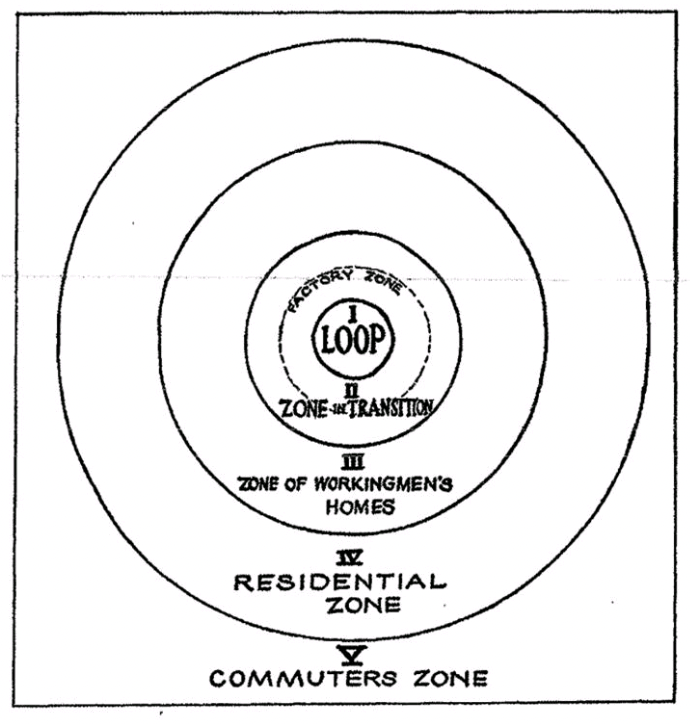
\includegraphics[width=30em]{burgess_model}
\end{center}

\subsubsection{Hoyt's sector model}

Between 1925-1939, the depression and economic crisis affected the US and less people were willing to move there. Thus, Hoyt was theoritising of a model where cities grow slowly, and the car plays an increasingly important role.

The sector model reflected the strong core (CBD) around which sectors are organised. When the city grows, or a certain group of people grows, these sectors grow outwards. There is a focus on class, rather than group of migrants.

\begin{center}
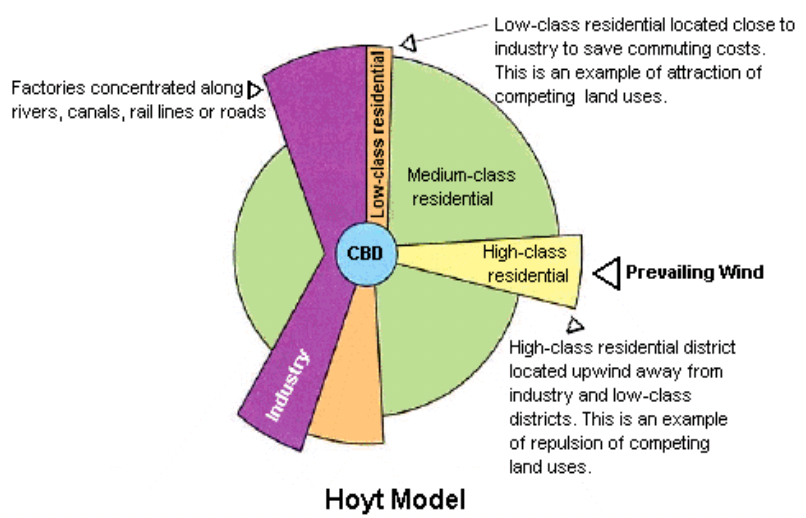
\includegraphics[width=30em]{hoyt_model}
\end{center}

\subsubsection{Harris and Ullman's multi-nuclei model}

A multi-nuclei model, where cities have a CBD but also other strong areas, with business (eg. river side industries) and other institutions (eg. universities).

\begin{center}
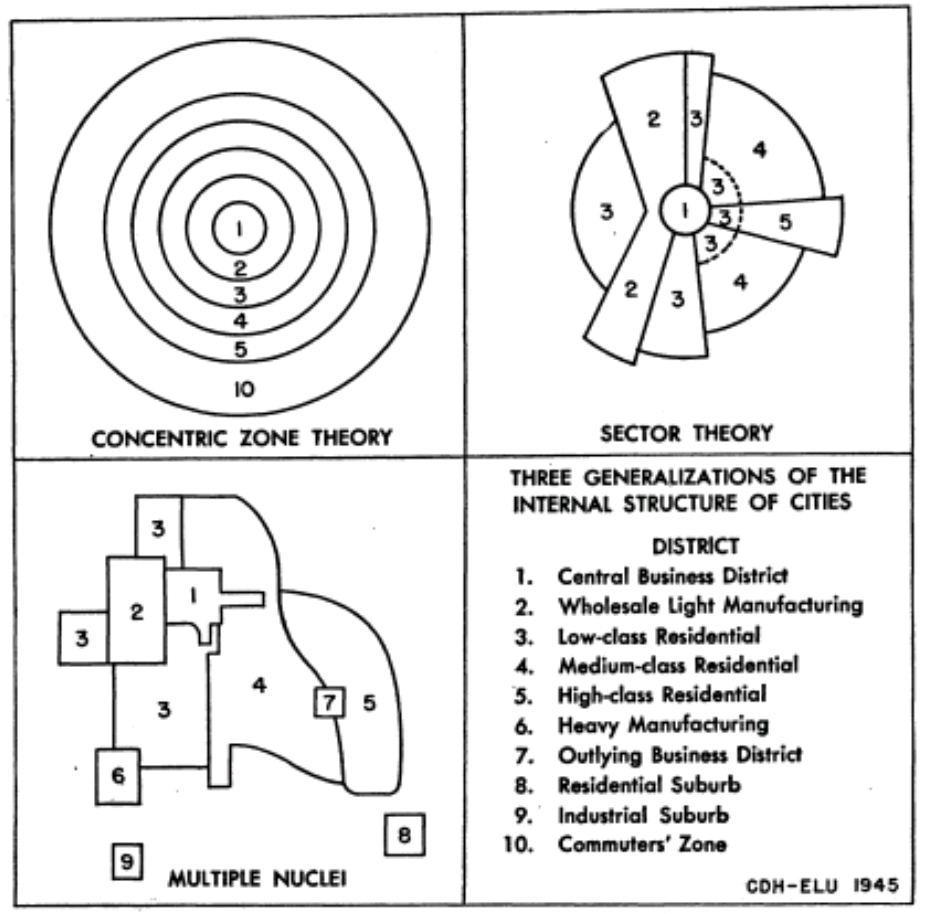
\includegraphics[width=30em]{harris_ullman_model}
\end{center}

\subsubsection{Alternative models}

The British city (Kearsley), the Chinese city (Burns), the African city, (De Blij), LA in 1990s (skid row, gated suburbs, Davis), the post-socialist city (Tallinn).

\subsubsection{Conclusion of classic land use models}

\textbf{Local features impact urban form} (topography, water bodies, prevailing wind direction, economic base of the city, migration patterns...) and \textbf{local policies impact urban form} (transport system, state interventions in housing, restrictions on mobility, strategies to counter inequalities...)

Thus, every model of urban form has its birthmarks, and is from a specific place and time. They need to be situated as such. We also need to \textbf{provincialise} theories about urban form and growth.

\subsubsection{Exam question - classic land use models and alternatives}

Exam question 2016: The figure below describes the model of the South African post- apartheid city by Christopher (2001). You can assume that the rich live in low density suburbs; the poor in high density suburbs and flats and hostels for male workers. +++ is a rail line; ---- represents a main road. Which elements of Burgess’, Hoyt’s and Harris and Ulman’s models of urban land use do you recognize in this model? (/5)

\[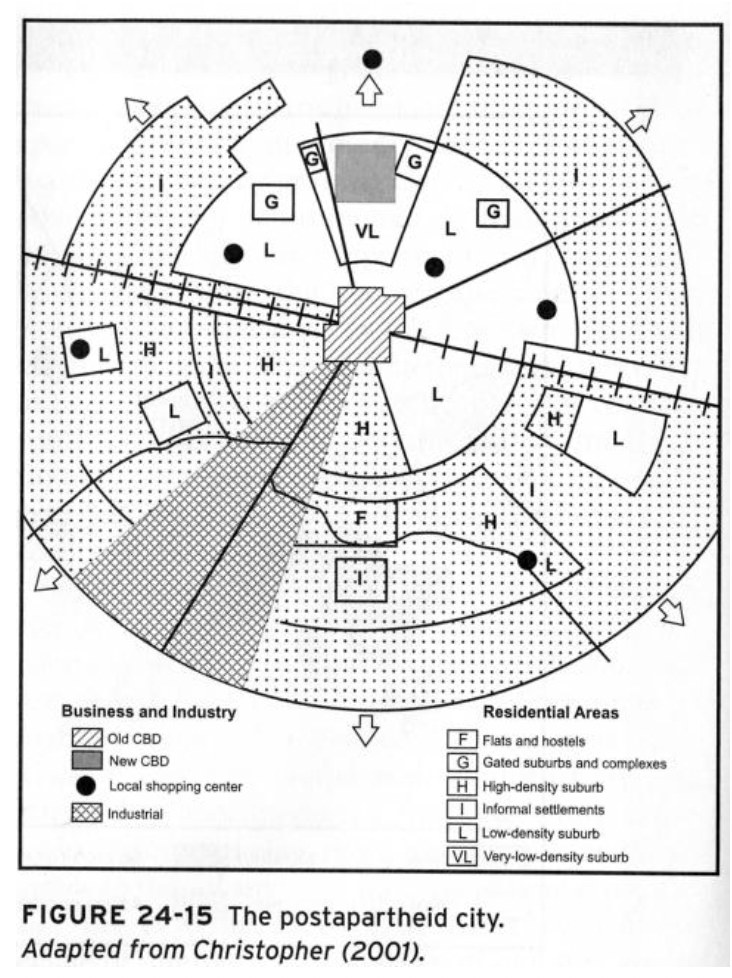
\includegraphics[width=15em]{examq_apartheid_model}\]

\subsection{Patterns of segregation}

\subsubsection{Massey and Denton’s five dimensions of segregation}

Segregation here is focused on \textbf{residential segregation}. It is the degree to which two or more groups live separately from each other, in different parts of the urban environment. Massey and Denton’s (1988) describe five dimensions of segregation: evenness, exposure, concentration, centralisation, and clustering.

\begin{outline}
	\1 \textbf{Evenness} is the differential distribution of two social groups, among areal units in a city; a minority group is said to be segregated, if it is unevenly distributed over a given area.
	The \textbf{index of dissimilarity} measures the unevenness in population across space. If an index is low, it means that the population is evenly distributed (ie. less segregation), whereas if an index is 100, the population is unevenly distributed (ie. high segregation). 
	\1 \textbf{Residential exposure} is the degree of possibility of interactions or contact, between minority and majority groups within geographic areas of the city; the degree of which these groups confront each other by virtue of sharing a common residential area
	\1 \textbf{Concentration} is the amount of physical space occupied by a minority group in the urban environment; groups that occupy a small share of the total area within a city are said to be residentially concentrated
	\1 \textbf{Centralisation} is the degree to which a group is spatially located near the centre of an urban area
	\1 \textbf{Clustering} is the degree of spatial clustering exhibited by a minority group, ie. the extent to which areal units inhabited by minority members adjoin one another, or cluster, in space
\end{outline}

\subsubsection{Scale matters}

Looking at segregation at different scales, give you very different results as to how segregated a city is. 

\begin{center}
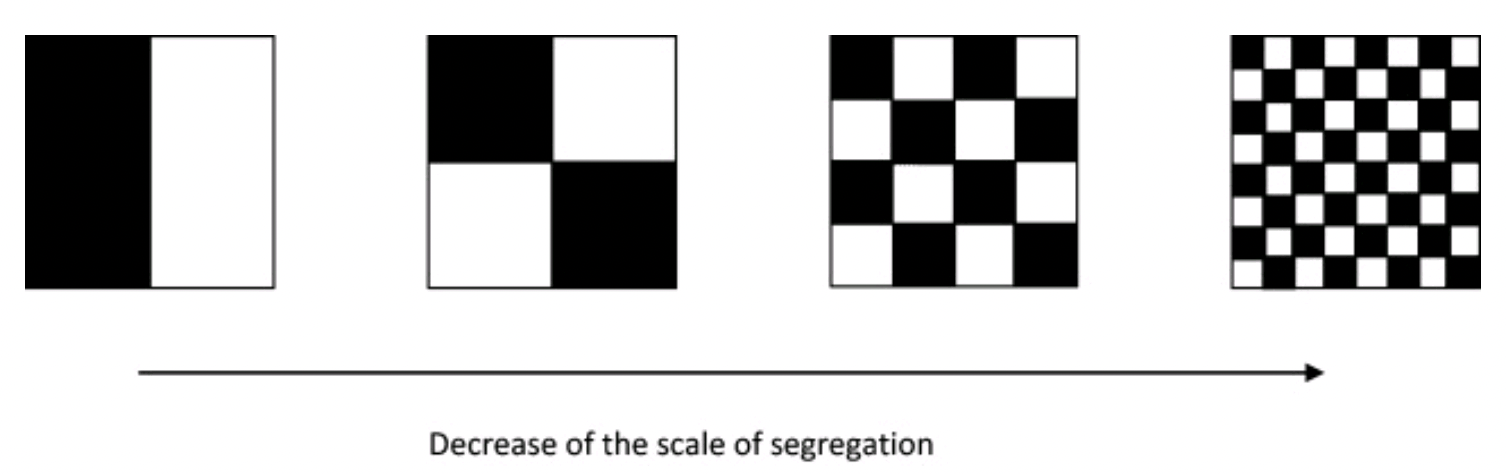
\includegraphics[width=30em]{segregation_scale}
\end{center}

\subsubsection{Exam question}

Exam question 2017: Use the three most relevant dimensions of Massey and Denton’s (1988) five dimensions of segregation to discuss socio-economic segregation in Brussels. Define each dimension of segregation you are using.

\[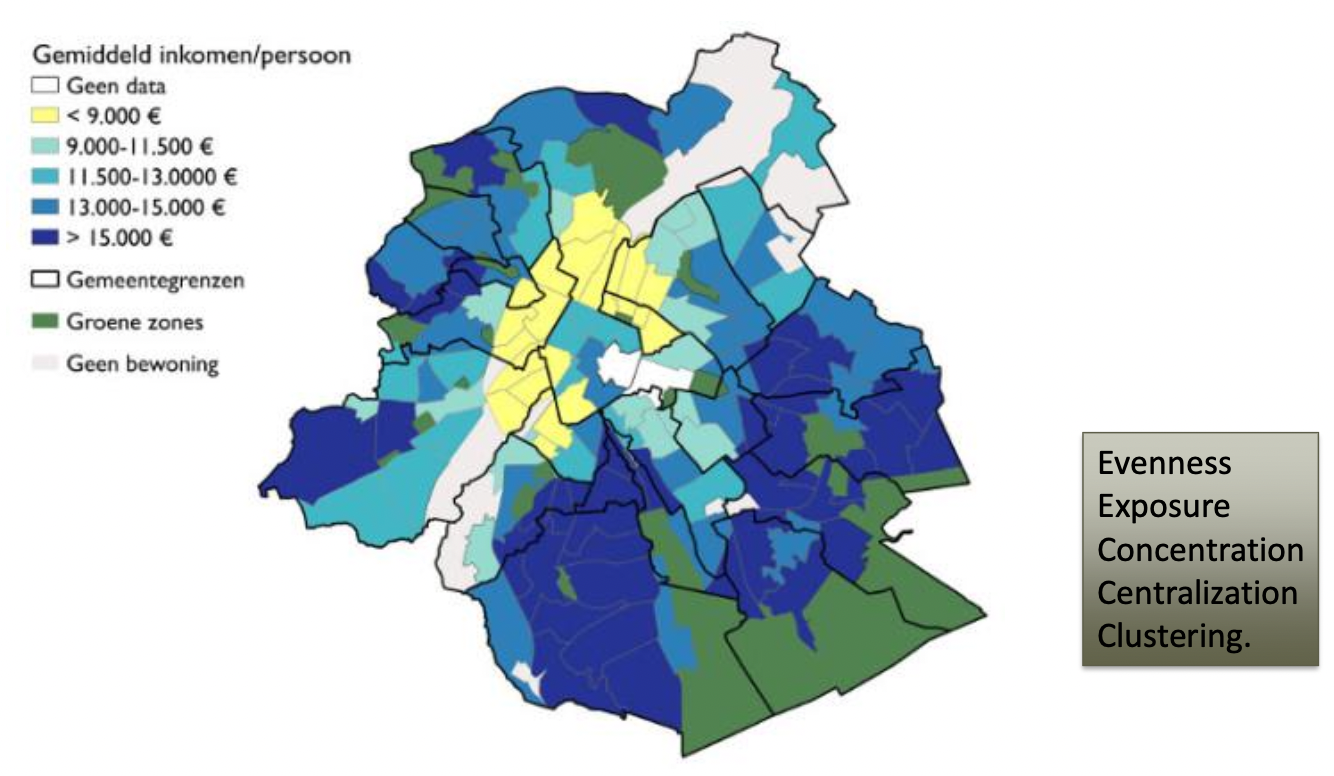
\includegraphics[width=30em]{examq_segregation_dimensions}\]

\subsection{Causes of segregation}

Why do different population groups occupy different parts of the city? There are many threads of geographers, with different opinions.

\begin{outline}
	\1 \textbf{Quantitative spatial geography}
	\1 \textbf{Ecological models} of the city
		\2 eg. ``urban metabolism'', ``natural forces''. It views the urban environment as a natural area, with a homogeneous character, characterised by a pattern of expansion (physical growth of the city) $\rightarrow$ competition (among land uses) $\rightarrow$ invasion (of the most desired parts of the city) $\rightarrow$ succession (of existing land uses)
	\1 \textbf{Radical-Marxist geography} 
		\2 Aims to understand the flow of capital, and the accumulation regime; how segregation fits within the accumulation of capital (Harvey)
		\2 The ecological models are considered to be mechanistic, ideological and devoid of ethical content
	\1 \textbf{Neo-Weberian} approach
		\2
	\1 \textbf{Behavioural geography}
		\2 Based on people's reasoning and preferences around living in a certain environment over another; there is a focus on the demand side of the housing market, which is closely tied to the family life-cycle
		\2 It can be done with an ethnic lens
	\1 \textbf{Post-modern geography}
		\2 The meaning of housing, and how this affects one personally, because housing is not just structural, but also about feeling at home
		\2 Raises questions like, what does moving to the suburbs do to a middle-class family? how does social mobility impact people? why do gentrifiers move back to the city centre?
		\2 It's all about having an identity, and how people understand and distinguish themselves from one another; gentrification is something that's promoted by the cities
\end{outline}

\[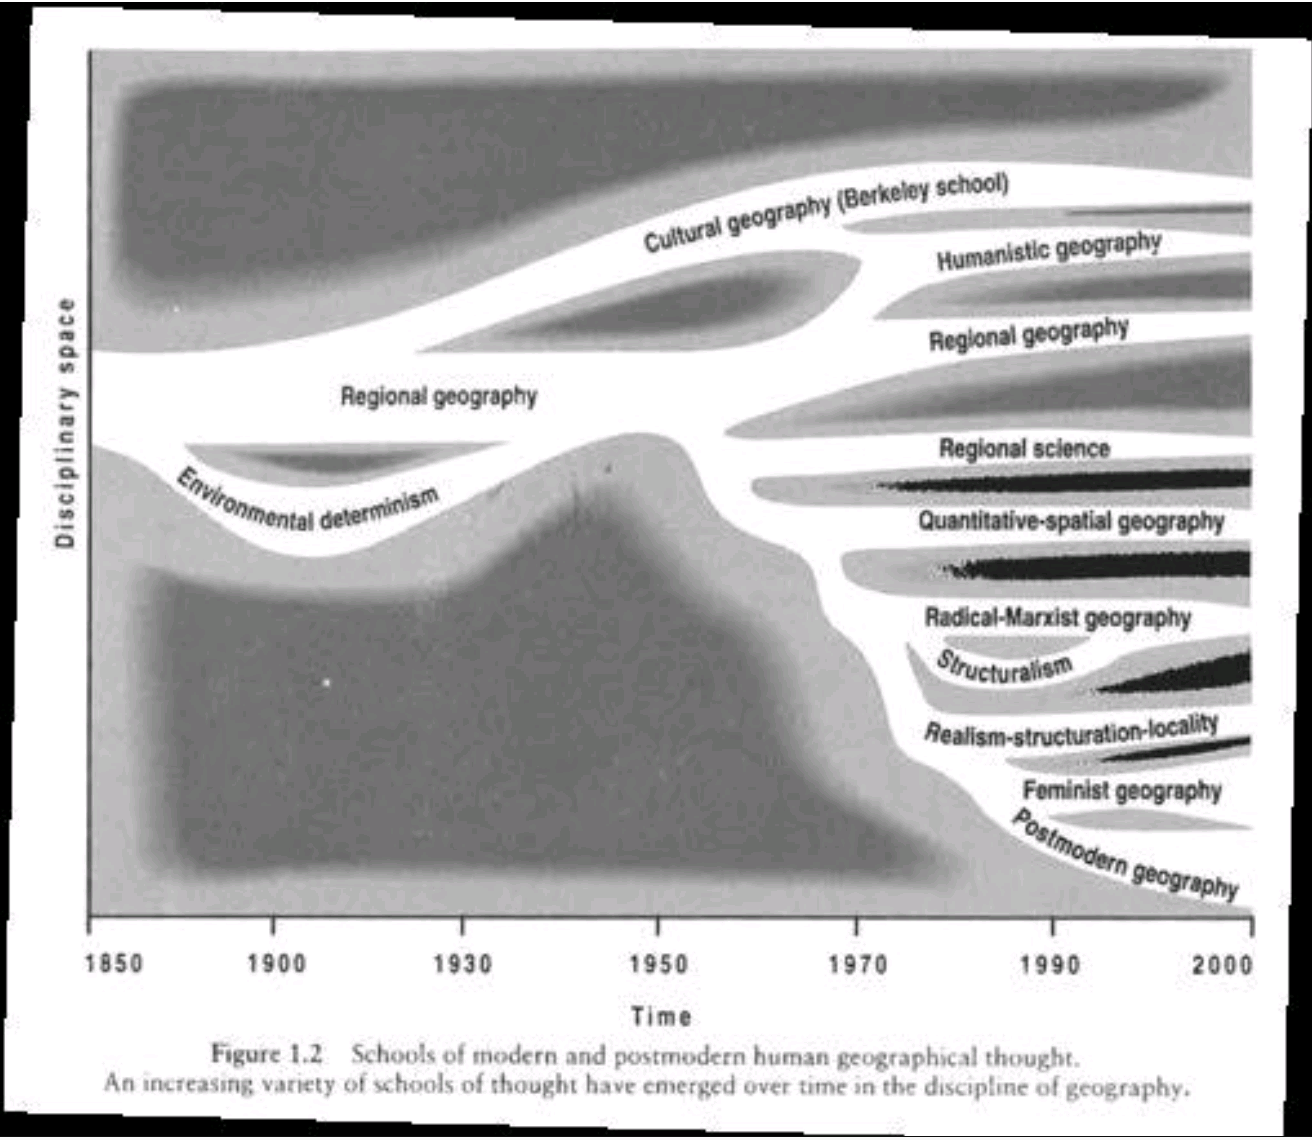
\includegraphics[width=30em]{geographer_types}\]

\subsubsection{Exam question}

Exam question 2017?: Below, you can find a map with the distribution of people of Turkish and Moroccan origin in the city of Antwerp. How would urban geographers from different schools of thought explain the patterns on the map? Refer to at least three traditions.

\[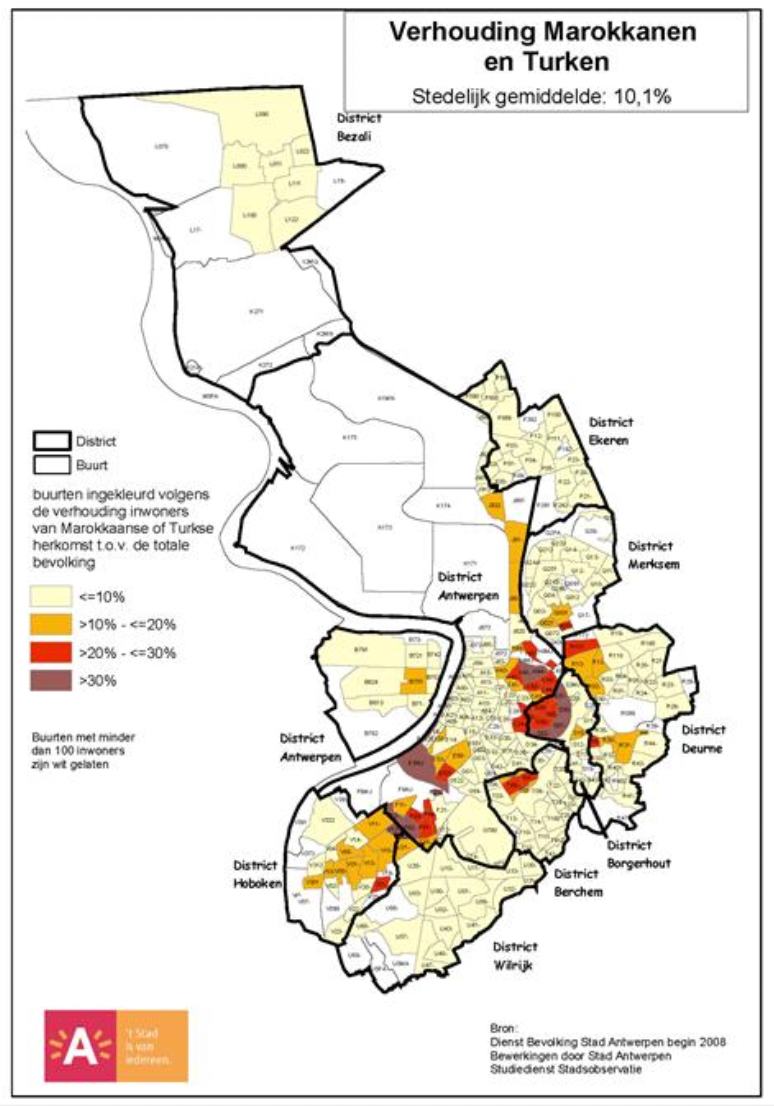
\includegraphics[width=20em]{examq_segregation_causes}\]

%%%%%%%%%%%%%%%%%%%%%%%%%%%%%%%%%%%%%%%%%%%%%%%%%%%%
%																	LECTURE 5
%%%%%%%%%%%%%%%%%%%%%%%%%%%%%%%%%%%%%%%%%%%%%%%%%%%%

\section{Neighbourhood effects and living with diversity}
\textit{November 8th, 2021 - Nick Schuermans}

\subsection{The ideal of social mix}

The ideal of mixed neighbourhoods has been on political agendas for a long time.
It is supposed that segregation has a negative effect on disadvantaged people (low-income, low-skilled), such that a disadvantaged person suffers more when living in a neighbourhood stricken by poverty, than in a neighbourhood without these ailments.

Different groups have different reasons for wanting social mixity: 

\begin{outline}
	\1 The \textbf{capitalist bourgeoisie} are afraid that the concentration of certain populations in a certain areas in a city, would have negative effects like revolutions, and that socialist thinking would become dominant
	\1 The \textbf{utopian socialists} were scared that the concentration of labourers would make it harder to create an egalitarian society
\end{outline}

The idea of social mixity is still dominant today and is high on the political agenda, worldwide, and across the whole political spectrum. Overall there are concerns about how the concentration of disadvantaged people and people of foreign origin affect \textbf{social mobility and cultural integration}.

\subsubsection{Examples of social mix}

\begin{outline}
	\1  Brussels Capital Region: ``Contrary to the American city, the ideal type for the European city is based on a mix of functions and people'' $\rightarrow$ ideal cities require a mix of people (poor, rich, local, foreign), and of type (residential, commercial, offices, etc.). The concentration of disadvantaged people in one area, makes it harder for these populations to be socially mobile, and they would be better off if they were living in a mixed income population
	\1 Ghent: attracting people with high-earning jobs will create a greater tax base, which will provide more capital to invest in the neighbourhood/city
	\1 Antwerp: regulation/efforts to prioritise a certain type of housing, ie. single family dwellings over smaller units, in order to attract more single families with higher income
	\1 UK: Housing Market Renewal (HMR), neighbourhoods mainly inhabited by disadvantaged people were plagued by demolition projects and construction of new dwellings. The idea is to transform the neighbourhoods, so that the inhabitants are no longer disadvantaged by their it, and make it easier for people to climb out of poverty
	\1 USA\marginpar{cfr. Slater}: Cabrini Green in Chicago, many apartment blocks were torn down and new houses built, to attract a middle class in a neighbourhood previously inhabited exclusively by disadvantaged
	\1 South Africa: using social mix and spatial integration to increase socio-economic opportunities
\end{outline}

Given the vast attempts at social mix, we ask ourselves: \textbf{is it possible to create socially mixed neighbourhoods, and do we want to?}

\subsection{Is social mix feasible?}

Policies like HMR (Housing Market Renewal) actually end up shifting the poverty elsewhere spatially, and do not solve the issue at the root. A metaphor is the waterbed effect, the idea that ``moving chairs on the deck of the Titanic' will only relocate the problem rather than fix it.

Gentrification comes with displacement, such that low-income, low-skilled people leave gentrified cities like Brussels, towards cheaper and more industrial, disinvested areas. Clusters of highly educated people converge towards Brussels, whereas cluster of low-income  concentrate in industrial/manufacturing areas such as Charleroi.
This illustrates the ``moving chairs on the Titanic'', where the disadvantaged are moved around within Belgium, but still exist, and their condition does not change. 

$\Rightarrow$ Thus, trying to create a social mix in some parts of the city (or country), displaces people and shifts poverty elsewhere, and ends up creating concentrations of poverty `down the street', eg. in Charleroi.

\textbf{Inclusionary housing/ zoning} in Cadix, Eilandje (Antwerp) is comprised of:
\begin{outline}
	\1 25\% social housing, including 15\% rent and 10\% buy
	\1 50\% ``affordable''
	\1 25\% ``residential''
\end{outline}

The mixes subsidised housing with non-subsidised. The city could have chosen to make more money by selling off the land to private developers, but chose to do otherwise, and impose a certain amount of social housing.

\textbf{So, is social mix feasible?} Yes, and projects that encourage social have integrated different populations, but it is hard to do in a situation where the market is dominant.

\subsection{Is social mix desirable?}

\subsubsection{Neighbourhood effects}

The assumption of neighbourhood effect is that ``where you live affects your life chances'' (Slater, 2013), and that ``impoverished neighbourhoods $[$could$]$ make their residents worse off'' (Friedrichs, 1998).

Different geographers have been asking different research questions (eg. ethnic cultural vs. socio-economic), and using different methods (qualitative vs. quantitative data, surveys), to understand neighbourhood effects.

Every study on neighbourhood effects bear birthmarks. It matters where a study takes place and studies need to be \textbf{provincialised and contextualised}.. 
Literature on the effects of segregation in the USA has been used to influence policy in Eastern Europe, but the context is different - for one, segregation in the USA is stronger than it is in Europe, where the welfare state is much more developed. When it comes to poverty, and the eradication of poverty, this contextual difference is important, and the ideologies can not always be transferred as-is. 

\subsubsection{Why it could matter where you live}

Seven arguments for why it could matter whether you are a disadvantaged person living in a disadvantaged neighbourhood, or in a mixed neighbourhood.

\begin{outline}
	\1 \textbf{Social network argument}: social capital is the connections between individuals, and networks the norms of reciprocity and trustworthiness that arises from them
		\2 Argument: mixed neighbourhoods will create connections, such that poor people are better off
		\2 Mixing people creates \textbf{bonding capital} between socially homogeneous people, eg. intra-ethnic, and \textbf{bridging capital} between socially heterogeneous people, eg. inter-ethnic
		\2 But
			\3 Increased mobility leads to \textbf{human extensibility}, leads to more networks and bonds outside the neighbourhood, especially at work or through kinship
			\3 Parallel lives: will drawing white families to Molenbeek help the people currently living there? Such people already have a social network outside of the neighbourhood, with people with the same social class, education status, etc. Thus, the middle class attracted to the neighbourhood will create connections with people similar to them, outside. This defeats the purpose of bringing middle class in, in the first place
			\3 Risks disrupting strong ties and bonding capital. Residents living in disinvested parts of the city, fall back on each other, ie. use bonding capital. Creating a mixed neighbourhood, by attracting the middle class, will displace the bonding capital that exists
			
	\1 \textbf{Underclass argument}:
		\2 \textbf{Structuralists} claim that poverty exists because of structural forces in a declining economic base (eg. move from fordist to post-fordist society, leading to lack of employment)
		\2 \textbf{Culturalists} claim that poverty exists because of a culture of poverty, with attitudes and behaviours that keeps people in their poverty. The ghettos (ie. neighbourhoods with concentration of disadvantaged people), with unemployment, vice, crime, addiction, disfunction, exist because of the \textbf{socialisation effects} (peer group effects, lack of adult role models) and the physical infrastructure and \textbf{institutional networks} within the neighbourhood
		\2 But
			\3 Causality: neighbourhoods with high concentration of drug use are located in the disadvantaged neighbourhoods; is this due to an uneven policing of disadvantaged neighbourhoods?
			\3 Socialisation outside neighbourhood facilitated by the internet, and people can connect via distance to people and media
	
	\1 \textbf{Social cohesion argument}: living in a neighbourhood with a high concentration of foreign speakers, will not acquaint you with the new country's language and norms, and this will make it harder to climb the social ladder. $\Rightarrow$ Ethnic segregation and socioeconomic mobility arguments for creating social cohesion
		\2 But
			\3 Mobility: is the neighbourhood the only place that such people can acquaint themselves with a new culture? There are many domains: home, work, leisure activities, where social mixing can happen outside the neighbourhood
			\3 Importance of local culture: protective spaces exist to give people a safe place to be, especially when they just arrive

	\1 \textbf{Local services argument}: a presence of the middle class will attract services, like banks and ATMs, and prevent food deserts. Mixed neighbourhood will attract a diverse set of shops and services
		\2 But
			\3 More differentiation will also lead to a differentiated demand: as diversity of people and businesses increase, some might not find what they are looking for; businesses might cater only to the middle class, and not the disadvantaged or ethnic groups, and thus displace the shops that previously existed and catered to low-income
			\3 Specialised services in arrival neighbourhood: will specialised shops and services (Thai, African...) remain?
			\3 Ethnic entrepreneurship will be overshadowed

	\1 \textbf{Political argument}: mixed neighbourhoods will be higher on the political agenda, because middle class people are more listened to or have connections to politicians. 
		\2 But, why do politicians not listen to the low-income populations in the first place?

	\1 \textbf{Spatial mismatch argument}: 
		\2 Concentration and clustering: in which part of the city is poverty concentrated? There is a mismatch between the location where people live, and where they could work (ie. where low-skilled jobs are available). 
		\2 But,
			\3 Public transport tends to be better in Western Europe, giving greater spatial mobility
			\3 The language divide can make it difficult to get a job in your area, especially in Brussels which speaks three languages. Do you need a specific language competency?
	
	\1 \textbf{Stigmatisation argument}: Teachers, businesses, employers come into neighbourhoods with a stereotype/stigma, and will not give as good chances to the people living there than otherwise
\end{outline}

\subsection{What about the privileged?}

We will never know! Ref. slides.

\subsection{Conclusion}

The concept of social mix is not very convincing. Gentrification simply moves disadvantaged populations to other parts of the city, which could be much worse, not provide the same services, and break social ties. 

When thinking about promoting social mix policies, we need need to ask:

\textbf{For whom?}
Why do we want to create a social mix? is it in the advantage of the underprivileged, or the privileged? for ethnic minorities, or majorities? for newcomers, or settled residents?

and, 

\textbf{Where and on what scale?}
The statistical units used to analyse segregation matters, are we looking at the city or regional scale? And where, only in disadvantaged neighbourhoods? only in gentrifiable, disadvantaged neighbourhoods? 
Why are we only concerned with disadvantaged neighbourhoods, and not other municipalities where we could ask whether it is worth creating diversity there.

and,

\textbf{Why?}
To counter poverty? To stimulate integration? There might be less costly, more effective policy alternatives than social mixing.
To counter racist stereotypes? To improve the local tax base? This uses the interest of poor people as rhetoric.

%%%%%%%%%%%%%%%%%%%%%%%%%%%%%%%%%%%%%%%%%%%%%%%%%%%%
%																	LECTURE 6
%%%%%%%%%%%%%%%%%%%%%%%%%%%%%%%%%%%%%%%%%%%%%%%%%%%%

\section{Cultures of urban research}

%%%%%%%%%%%%%%%%%%%%%%%%%%%%%%%%%%%%%%%%%%%%%%%%%%%%
%																	LECTURE 7
%%%%%%%%%%%%%%%%%%%%%%%%%%%%%%%%%%%%%%%%%%%%%%%%%%%%

\section{Urban cultures}

%%%%%%%%%%%%%%%%%%%%%%%%%%%%%%%%%%%%%%%%%%%%%%%%%%%%
%																	LECTURE 8
%%%%%%%%%%%%%%%%%%%%%%%%%%%%%%%%%%%%%%%%%%%%%%%%%%%%

\section{Transport and cities: a historical hegemony}

%%%%%%%%%%%%%%%%%%%%%%%%%%%%%%%%%%%%%%%%%%%%%%%%%%%%
%																	LECTURE 9
%%%%%%%%%%%%%%%%%%%%%%%%%%%%%%%%%%%%%%%%%%%%%%%%%%%%

\section{Critical perspectives on urban transport}

%%%%%%%%%%%%%%%%%%%%%%%%%%%%%%%%%%%%%%%%%%%%%%%%%%%%
%																	SEMINARS
%%%%%%%%%%%%%%%%%%%%%%%%%%%%%%%%%%%%%%%%%%%%%%%%%%%%

\section{Seminars}

\subsection{Seminar 1: World/Global cities}
\textit{October 19th 2021, David Bassens}


\subsection{Seminar 2: Diverse Cities}
\textit{November 18th 2021, Nick Schuermans}

\subsubsection{Muster et. al, ``Socioeconomic...''}
\begin{outline}
	\1 Spatial segregation hypothesis:
		\2 
	\1 Discussion
		\2 Assumption that socio-economic segregation is a cause, not a symptom; implies that the problem is concentration of classes (ie. space), and the solution is social mix; 
		\2 Local context and time are important for understanding the socioeconomic segregation in a given place
		\2 Does not mention capitalism
	\1 Discussion questions
		\2 If you reduce spatial segregation will this reduce socio-economic inequality?
		\2 Why do researchers of urban social mixing/spatial segregation place an emphasis on diversifying the residential housing stock? Can you think of other urban spaces in which socio-spatial mixing can occur?
\end{outline}

\subsubsection{XXX, ``Paradoxes of (post-) socialist segregation: XXX''}
\begin{outline}
	\1 Cities were more segregated before WWII, than during socialism; 
	\1 Highly sensitive to historical context
		\2 Warsaw: in WWII city was destroyed and communities displaced; socialist focus was to reconstruct; socialist regime had patterns of meritocracy (higher position in state = better housing); high income polarity between highly educated, middle class, and others
	\1 In global cities, income polarity has increased but  decreasing social segregation and concentration; this is rooted in the pre-socialist past of these cities
		\2 You might expect global cities to be wealthier and thus less socio-economic inequality, but this is not the case; actually the opposite
	\1 Discussion questions
		\2 If there is an increase in income inequality, but decrease of segregation, what does this mean for the city?
		\2 Does this mean that less segregation is always a positive indicator in cities?
\end{outline}

\subsubsection{Shien and Xiao, ``Emerging divided cities in China: socioeconomic segregation in Shanghai, 2000-2010''}
\begin{outline}
	\1 Economic restructuring, neoliberalisation, globalisation changed role of household type and lifestyle
	\1 	Socio-economic segregation factors
		\2 Housing reforms: abolition of welfare housing system, privatisation, opening of housing markets (commodification) $\rightarrow$ increase in housing price, development of housing in the suburbs
		\2 Educational composition
	\1 Discussion questions
		\2 
\end{outline}


\subsubsection{Visser et. al, ``''}
\begin{outline}
	\1 How young people's experience of the neighbourhood important for understanding how the neighbourhood works as an entity?
		\2 Lived experiences affect socio-spatial behaviour and life paths of people 
		\2 Youths have a view that differs from hegemonic discourse; neighbourhood effect studies should avoid overly simplistic descriptions of youths in deprived neighbourhoods; this paper gives agency to youths 
		\2 Youths are aware of their neighbourhood features and insights could be useful for policy makers
	\1 Discussion questions
		\2 What should be the role of youths in the neighbourhood effect research?
		\2 How do we define good (decent) social networks?
\end{outline}

\subsubsection{Schuermans et. al, ``Geographies of whiteness and wealth: white, middle class discourses on segregation and social mix in Flanders, Belgium''}
\begin{outline}
	\1 Is the middle class ready and willing to assume the role that policy makers assign to them through their social mix strategies
\end{outline}


\subsection{Seminar 3: Cultural Cities}
\textit{December 9th 2021, Bas van Heur}


\subsection{Seminar 4: Urban Transport and Mobility}
\textit{December 16th 2021, W. Keblowski}


%%%%%%%%%%%%%%%%%%%%%%%%%%%%%%%%%%%%%%%%%%%%%%%%%%%%
%																	READINGS
%%%%%%%%%%%%%%%%%%%%%%%%%%%%%%%%%%%%%%%%%%%%%%%%%%%%

\section{Readings}

\subsection{Polarisation in World/Global Cities}

\subsubsection{Hamnett, \textit{The changing social structure of global cities: Professionalisation, proletarianisation or polarisation}}

\begin{outline}
	\1 There are three trends studied: professionalisation, proletarianisation and polarisation. These concepts have shaped the social structure of global cities, and the paper aims to understand whether there is a dominant trend
	\1 \textbf{Professionalisation} refers to an increase in ``professionalised'' occupations, with an increase in professional, managerial and technical workers, some on high income. Professionalisation started as a result of changes in the industrial structure (from industrialisation to a post-industrialisation era starting in the 1970s).
	\1 \textbf{Proletarianisation} is the increase in de-skilled jobs, as a result of changing industrial structures (basically the opposite of professionalisation, as a result of industrial structure changes).
	\1 \textbf{Polarisation} is the growing gap between the top and bottom ends of the occupational and income distribution, where the middle in shrinking.
	\1 Society went from a pre-industrial (pre-1840s), to industrial (1840s) and \textbf{post-industrial society} (PIS, 1970s). 
		\2 It shifted from a society dominated by manufacturing employment, to one dominated by the service sector and drastic decrease in manufacturing employment. PIS could be expected to give rise to de-proletarianisation (decline in working class) due to machinery and innovation replacing manual labour. On the other hand, capitalism generates technical innovation that could replace high-skilled labour, which would increase proletarianisation.
		\2 Researching the class structure of PIS shows that there is an upwards shift towards professionalisation, and that society is biased towards high-skilled labour (top and middle classes) rather than low-skilled (bottom class). Children with working-class parents and grandparents are now likely to be graduates and work in professional careers
		\2 However, the growth of professionalisation, and thus of the professional and managerial class, has been accompanied by an increase in income inequality and precarious work $\rightarrow$ polarisation
 \end{outline}

\subsubsection{May et. al, \textit{Keeping London Working: global cities, the British state and London's new migration division of labour}}

\begin{outline}
	\1 Instead of focusing on professionalisation and jobs at the top end of the market, this paper focuses on the bottom end and specifically on the character and composition of the people who work there (mostly  foreign-born and migrant labour). 
	It explores how state welfare, labour market, and migration policies have changed the labour market and increased the low-skilled labour demand, which is disproportionally taken up by foreign-born workers and new migrants.
	\1 It criticises Hamnett's work, saying that it focuses too much on professionalisation rather than polarisation
	\1 Regarding the state welfare policies, it did not protect wages or working conditions. Instead, Conservative governments tried hard to secure a competitive economic advantage for Britain by labour market de-regulation and welfare restructuring. The British state actively tried to facilitate the recruitment of migrant labour, at the same time restricting people's welfare.
		\2 A significant proportion of the bottom of the labour force are migrants, working long and unsociable hours, for extremely low rates, without protection offered to native workers like the benefits system
	\1 Bottom-up initiatives, and places of faith have taken on the role of campaigning for worker's rights s
\end{outline}


\subsection{Urban segregation: patterns and causes}

\subsubsection{Pacione, \textit{Land Use in the City}, 2009}

\begin{outline}
	\1 Morphogenesis: the study of town-planning, and what causes the city to have the shape it does
		\2 Urban landscape can be divided in three elements: land use (the most susceptible to change), buildings (less susceptible to change because their use can change without the building changing), town plan (street layout, most resistant to change) (Conzen, 1960)
		\2 Town plan is the outcome to the visions and policies of individuals (eg. landowners) or agencies (eg. local planning dept) that have the power to change the urban landscape
		\2 Need to understand the background, motivations and actions of the major agents in the development of townscapes
	\1 Human ecology: stems from the Chicago school
		\2 ``Competition among land uses for space resulted in the invasion of the most desired parts of the city and eventually the succession of existing land uses by a more dominant activity''
		\2 ``Natural'' areas would evolve, based on class and ethnicity 
		\2 \textbf{Burgess' concentric zone} model is an ideal type, with known limitations (which is why applying it to other cities can be difficult)
		\2 Public redevelopment scheme and government policies (eg. social housing), and gentrification of the inner-city, challenge the value of model today
		\2 \textbf{Hoyt's sectors}: urban land use starts at the city centre, around which the sectors are organised. The sectors grow only outwards. Critique is that it only represents residential housing and does not take into account class or ethnicity
		\2 Burgess' model focuses on the demand side of housing, whereas Hoyt's model focuses on the supply-side mechanisms whereby middle class housing develops in the periphery. Both are extremely simplistic
		\2 \textbf{Harris and Ullman's multi-nuclei}: the location and growth of the multi nuclei are based on factors such as, activities require specialised facilities, similar activities group together, some activities repel each other, and some activities must locate elsewhere than where is most convenient because of eg., high rent prices
		\2 Modern models: Mann's model of typical UK city, Kearsley's modified Burgess model, Vance's urban realms model, White's model of 21st century city
	\1 Political economy: seeking interpretations of urban change that reveals the structural forces underlying the observed land-use patterns
		\2 Capitalist societies, based on capital accumulation, are designed in such a way as to facilitate the transfer of profits and maximise the opportunities for investment $\rightarrow$ circulation of capital (Harvey)
		\2 Circuits of capital:
			\3 Primary circuit: the production process; surplus created during production is reinvested in primary circuit, or if there is not enough demand to produce more, in to the secondary and tertiary circuits
			\3 Secondary circuit: investment in fixed capital (built environment, real estate); profit is in the form of rent, or increased exchange value (sale price) 
			\3 Tertiary investment: in science and technology, ie. innovations to improve productivity, or labour capability (eg. health, education); this investment is usually made by the state
		\2 Contradiction between capital accumulation (provokes urban change and redevelopment) and the built environment (resists change)
\end{outline}

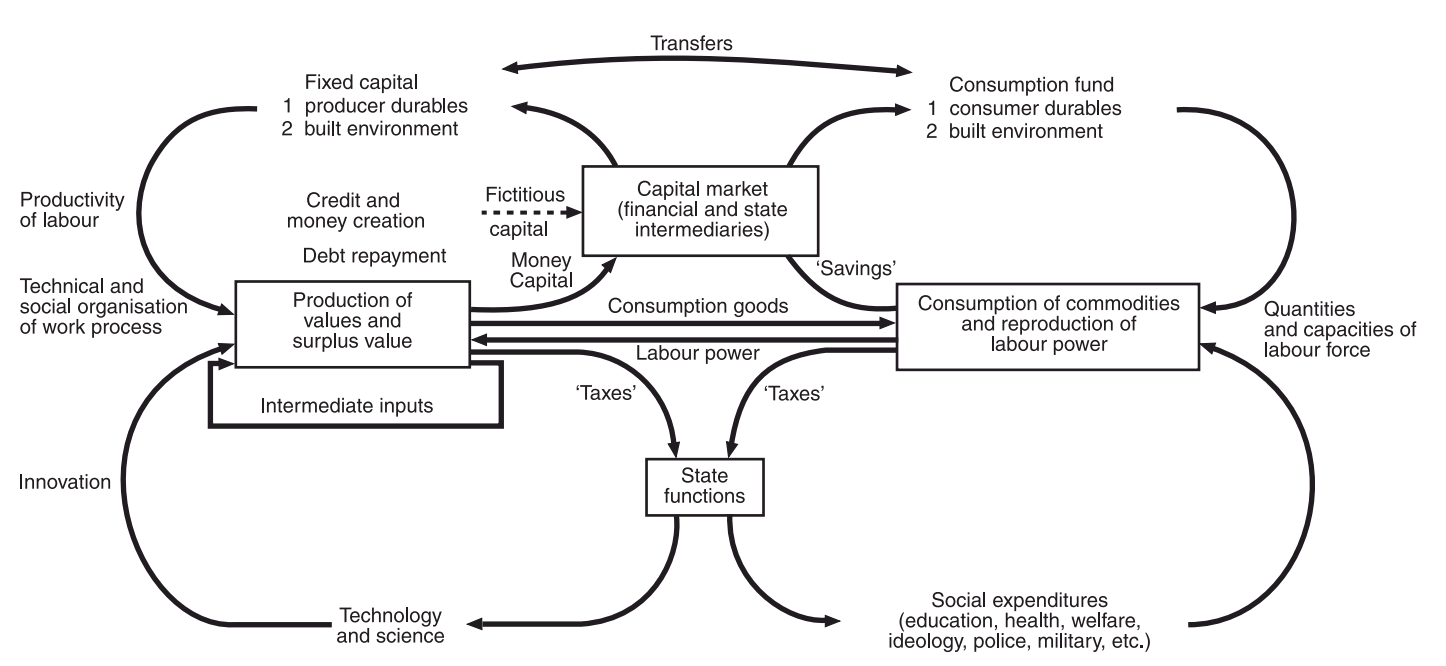
\includegraphics[width=\textwidth]{harvey_circulation_capital}

\subsubsection{Van Kempen, Sule Özüekren, \textit{Ethnic segregation in cities: new forms and explanations in a dynamic world}, 1998}

\begin{outline}
	\1 Segregation and concentration: \textbf{spatial segregation} is the residential separation of groups, ie. the degree of deviation from the uniform spatial distribution of all populations within a city. Spatial segregation implies \textbf{spatial concentration}, whereby one population group is disproportionately represented in a given space, compared to other groups
		
	\1 Disadvantages of spatial segregation and concentration
		\2 Living in a segregated/poor neighbourhood limits your opportunities in life (education, employment, health...)
		\2 Poverty has an effect on facilities (commercial and not)
		\2 Neighbourhood effects: the way the neighbourhood is viewed by others, and its stereotypes, contribute to self-fulfilling prophesies; this is a limited understanding, and is dangerous because it can lead to a lack of empathy towards those populations
		\2 Ghettos are ``institutionalised'': residents did not choose it for themselves, rather, they were coerced by society; residence is involuntary
		\2 \textbf{Underclass} ``suffer from prolonged labour-market marginality and have virtually no chance to alter this situation''. They're economically and politically isolated, usually have deviant or illegal behaviours, their lifestyle is one of survival and is different from that of the poor. Dangerous because it lumps together different populations, and normalises them
		
	\1 Advantages of spatial segregation and concentration
		\2 Existence and maintenance of social contacts is made possible by the concentration of like-minded people; it encourages cultures and norms that are not those of the mainstream society
		\2 Social networks allow people to support each other
	\1 Behavioural approach: explanations that include the preferences, perceptions and decision-making of the individual in housing and residential mobility
	\1 Ethnic-cultural approach: cultural differences between groups can help explain differences in housing conditions and residential patterns

\end{outline}

\section{Cultures of urban research}

\subsubsection{Barnes, \textit{The 90s show: culture leaves the farm and hits the streets}, 2013}

\begin{outline}
	\1 Urban studies originally described the city as a place devoid of culture, and in purely economic terms (work, production, economic activity, Marxist, rent gap, urban gatekeepers, uneven development). Culture entered the urban studies sphere in 1990s, when cultural studies, postmodernism, new cultural geography emerged
	\1 ``My intention is to examine the processes by which culture came into urban geography, and the particular forms it has taken'' (p. 480)
	\1 Histories of urban and cultural geography, and their relationship
		\2 Sauerian (Sauer) cultural geography: focused only on the rural as a place of culture; extensive field research with natives; the cultural landscape is more than the sum of its parts, taking a holistic view of the cultural landscape, implies that there is an `environmental determinism'; emphasis local cultural and was skeptical of metropolitan power;
		\2 Beginning of urban geography in mid-1950s: was the anti-thesis of Sauerian cultural geography; believed in modernity, analysis, model and system building, quantitative empirical methods; urban geography was a spatial science
			\3 Urban geographers wanted to analyse the effect of modernity in the city
			\3 Analysis was a key tool: breaking down problem into quantifiable subelements, that can be related to each other
			\3 ``Radical political economists'' like Harvey and Castells put the city at the heart of capitalism. This ignores all cultural elements
			\3 Saurian cultural geography lacked a political purpose (Engels' accounts of Manchester, Marx' Communist Manifesto)
	
	\1 Reconciliation between urban and cultural geography, stemming from debates in political economy, cultural studies, and reconceptualisation of cultural geography
		\2 Cultural cannot be ignored when studying the city; it was ignored by urban geographers (either spatial or radical geographers) notably because of the connotations of Sauer and cultural geography
		\2 Revamping of urban geography by culture:
			\3 Outside urban geography emerged cultural studies and postmodernism that theorised the relationship between culture and economy
			\3 New cultural geography emerges, and critiques and replaces Sauerian cultural geography; says that culture is everywhere, from the most mundane to the most spectacular
		\2 Cultural studies showed that one could analyse class and the economy, while still recognising values, ways of life, and emotional and political commitments outside the economy
		\2 There are many discussions and positions on postmodernism
		
	\1 Specific forms that the ``cultural turn'' is taking in urban geography
		\2 In 1990s, urban geography increasingly became urban cultural geography; there was a merging of culture and economy, and urban geography became both, not either/or
		\2 Public space\footnote{Harvey, 1989, Conditions of Postmodernity} has become increasingly commodified, culture is used to extract money
		\2 Urban cultural industries: located in the worlds most powerful metropolitan centres. The economy is defined by new cultural products, and cultural products are produced because they are economic commodities.
		\2 Gentrification: originally in the 1980s either an economic argument, the rent gap theory (Smith), or a cultural argument, the postindustrial middle class making lifestyle and consumption choices (Ley); now, it is about both
		\2 Economic services and innovation: economy and culture are intertwined, capitalism is taking a cultural turn as businesses focus on ``creation, fostering and distribution of knowledge''; this happens in the city because that is where the forces exist that allow culture to be inextricably linked with the economy
		\2 International immigration and transnationalism: both economic and cultural factors, and class, gender, ethnicity, influence what patterns, changes, and resistance exist with regards to migration
\end{outline}

\subsubsection{, \textit{}}

\begin{outline}
	\1
\end{outline}


%%%%%%%%%%%%%%%%%%%%%%%%%%%%%%%%%%%%%%%%%%%%%%%%%%%%
%																		EXAM etc.
%%%%%%%%%%%%%%%%%%%%%%%%%%%%%%%%%%%%%%%%%%%%%%%%%%%%

\section{Exam}

\href{https://bakexamenwiki.wordpress.com/urban-geography/?fbclid=IwAR1qxA_V_G9I3NVC_17dFMUmEMLisoLB-XfgdqZmQNxIsUydvhO_ZnCOFVU}{2021 Exam Questions}

\subsection{Urban segregation}

See lecture 4 slide 28

\if{false}

\subsubsection{, \textit{}}

\begin{outline}
	\1
\end{outline}


\fi

\end{document}